\documentclass[tc, manuscript]{copernicus}

\usepackage{booktabs}
\usepackage{multirow}
\usepackage{siunitx} 

\begin{document}

\title{Fountain scheduling strategies for improving water-use efficiency of artificial ice reservoirs (Ice stupas)}

\def\Authors{Suryanarayanan Balasubramanian\,$^{1,2}$, Martin Hoelzle\,$^{1}$Roger Waser\,$^{3}$}

\def\Address{$^{1}$University of Fribourg, Department of Geosciences, Fribourg, Switzerland $^{2}$University of
Applied Sciences and Arts, Luzern, Switzerland} \def\corrAuthor{Suryanarayanan Balasubramanian}
\Author[1,2]{Suryanarayanan}{Balasubramanian}
\Author[1]{Martin}{Hoelzle}
\Author[3]{Roger}{Waser}
\affil[1]{University of Fribourg, Department of Geosciences, Fribourg, Switzerland}
\affil[2]{Himalayan Institute of Alternatives, Ladakh, India}
\affil[3]{University of Applied Sciences and Arts, Luzern, Switzerland}

\correspondence{suryanarayanan.balasubramanian@unifr.ch}

\runningtitle{Scheduling AIR fountains}

\runningauthor{S. Balasubramanian}

\firstpage{1}

\maketitle

\begin{abstract}

  Artificial ice reservoirs (AIRs), also called ice stupas, are a climate-change adaptation strategy
  developed in the Indian Himalayas (Ladakh). With this technology, otherwise unused stream/spring water is
  stored in large ice towers during the winter. The surplus melt water generated in spring is used to
  satisfy irrigation water demands. Recent studies have shown that, during AIRs construction, over 75\% of
  the water sprayed is lost. We examine whether fountain scheduling strategies can reduce this
  water loss by building two AIRs under identical weather conditions but with different fountain scheduling
  construction strategies. Fountain scheduling was performed through an automation system computing recommended
  discharge rates using real-time weather input and location metadata. Fountain operation using scheduling
  strategies produced similar ice volume while consuming one-tenth of the water the unscheduled fountain used.
  Simulations converting unscheduled fountains into scheduled fountains showed a threefold improvement in water-use efficiency. Overall, these results show that automated fountain water supply
  management can increase water-use efficiency of AIRs and reduce their maintenance without compromising
  their meltwater production.

\end{abstract}

\introduction

Cryosphere-fed irrigation networks in arid mountain regions are completely dependent on timely availability of
meltwater from snow, glaciers, and permafrost \citep{immerzeelImportanceVulnerabilityWorld2020,
farhanHydrologicalRegimesConjunction2015, tveitenGlacierGrowingLocal2007}. With the accelerated decline of
glaciers due to climate change, these regions are experiencing seasonal water scarcity
\citep{hoelzleStatusRoleAlpine2019, xenariosAralSeaBasin2019, barandunStateFutureCryosphere2020}, which limits the output and duration of agricultural activities.

In Ladakh, a cold arid desert in northern India, a typical shortage of water occurs at the onset
of the agricultural season (April and May) until a sufficient and reliable supply of meltwater from glaciers
becomes available \citep{norphelSnowWaterHarvesting2015, nusserLocalKnowledgeGlobal2016,
vincentEnergyClimateChange2009}. 

To cope with this recurrent water scarcity, villagers have developed artificial ice reservoirs (AIRs; Fig.
\ref{fig:AIRforms}a). AIRs capture water during autumn and winter, freezing and holding it until
spring, when this water melts and flows down to irrigate the fields \citep{ipccChapterHighMountain2019,
vinceGlacierMan2009, clouseLadakhArtificialGlaciers2017, nusserSociohydrologyArtificialGlaciers2019}; thus retaining a previously unused portion of the annual flow and facilitating its use to compensate the decreased flow during the following spring.

A spirit of improvisation guides the construction strategy of AIRs, challenging their classification.
Construction strategies using fountain systems form AIRs which tend towards a
conical shape, whereas those strategies without fountain systems form flat sheets of ice. Therefore, in the present study, we classify AIRs 
based on whether or not these use fountain systems. AIRs using fountain systems are called ice stupas (Fig.
\ref{fig:AIRforms}c) and those without are called ice terraces (Fig. \ref{fig:AIRforms}b), according to the resulting shape of the respective AIRs. In the present work, we investigate the ice
stupa form of AIRs.

\begin{figure}[htb]
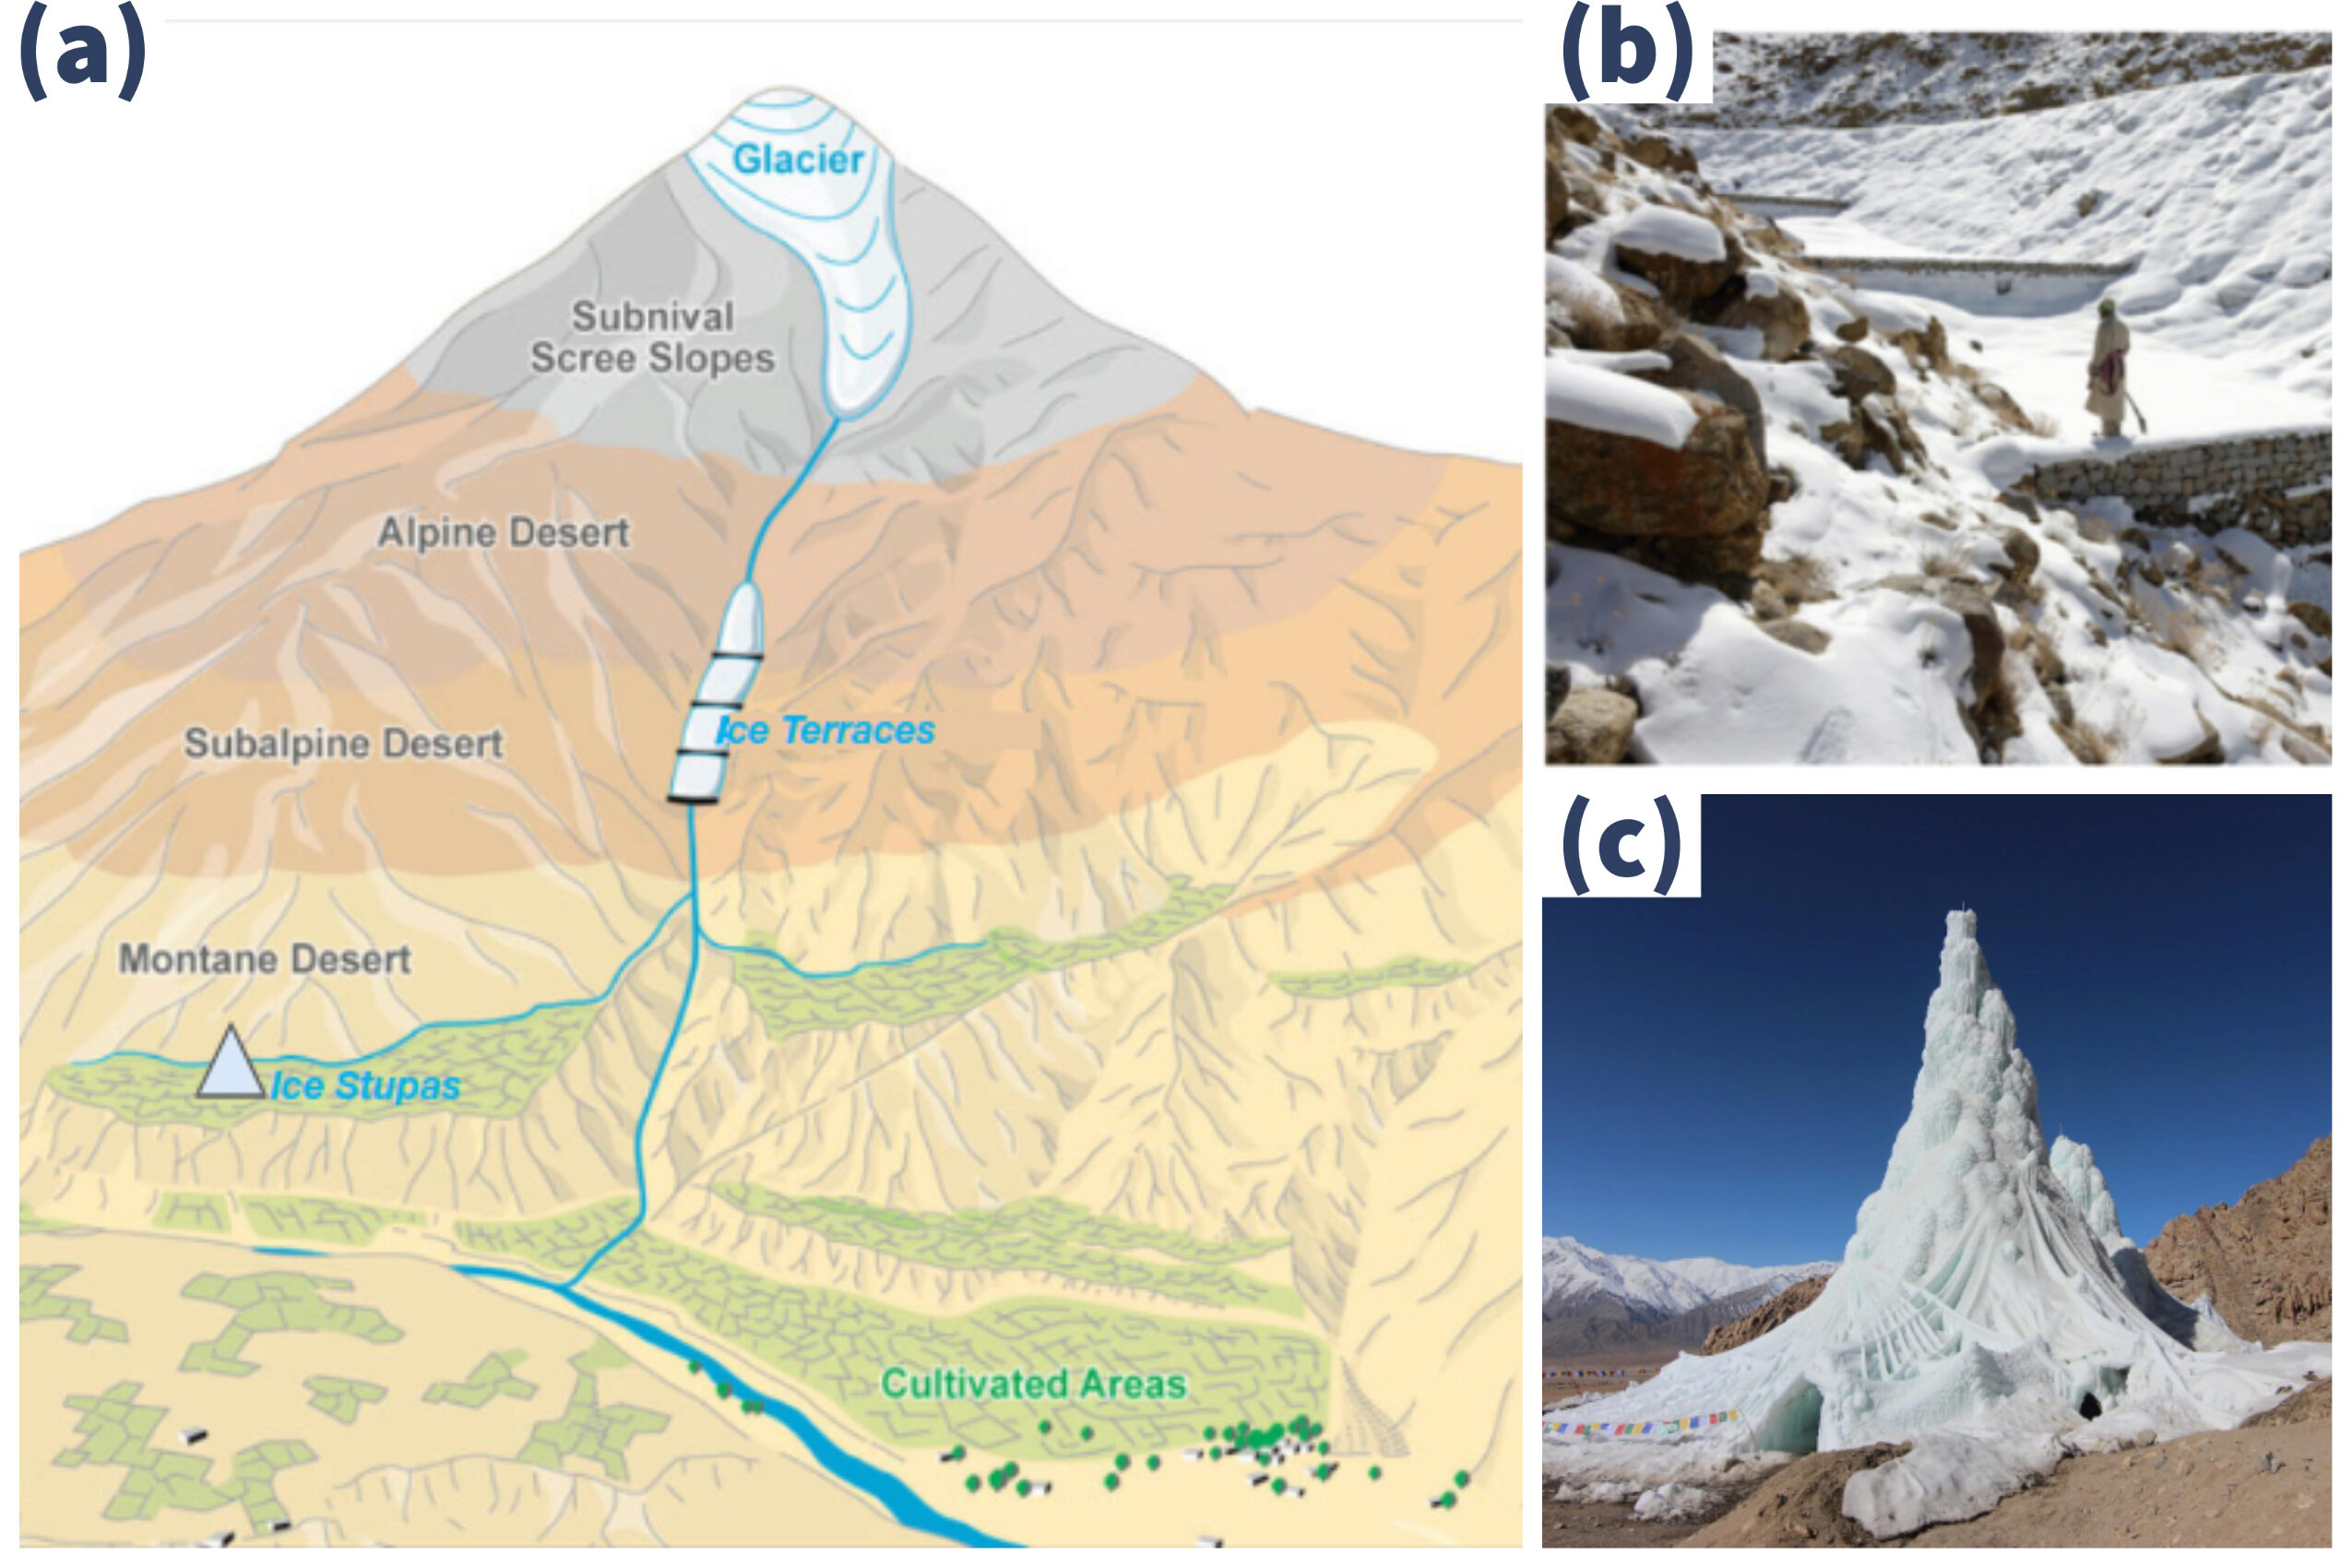
\includegraphics[width=12cm]{Figures/AIR_forms.jpg}

\caption{(a) Schematic overview of artificial ice reservoirs (AIRs) located at
altitudes between the glaciers and the irrigation networks in the cultivated areas; (b) ice terraces and (c) ice
stupas are located at higher and lower altitudes, respectively. Adapted from:
\cite{nusserLocalKnowledgeGlobal2016}}

\label{fig:AIRforms}
\end{figure}

Over the past decade, several ice stupas have been built to supplement the irrigation water supply of mountain
villages in India \citep{wangchukIceStupaCompetition2020, palmerStoringFrozenWater2022,
aggarwalAdaptationClimateChange2021}, Kyrgyzstan \citep{bbcnewsBrightArtificialGlacier2020}, and Chile
\citep{reutersConservationistsChileAim2021}. These AIRs are traditionally constructed by diverting springs or
glacial streams into fountain spray systems via embankments and pipelines. 

A common issue of AIR construction systems is fountain scheduling, namely answering the questions “when to spray?,” “how much?,” and “for how long?.”
Starting a fountain spray too early, spraying too much water, or running a fountain spray for too long might lead to
overwatering; at the very least, this practice wastes water. Similarly, starting the fountain spray too late,
spraying too little water, or not running the system for long enough might lead to underwatering and can cause
reduced ice volume or freeze the water supply pipelines.

Previous work \citep{balasubramanianInfluenceMeteorologicalConditions2022} has shown that traditional
construction systems suffer from overwatering. To avoid this issue, we need to understand
surface freezing rates, which can be calculated by means of the full energy balance model developed in
\cite{balasubramanianInfluenceMeteorologicalConditions2022}. This model requires an accurate estimation of
fountain spray radius to produce recommended discharge rates. In theory, we can estimate this by
modelling the projectile motion of water droplets using fountain characteristics such as aperture diameter and
discharge rate. In practice, this estimation depends also on the relative importance of wind-driven
redistribution effects. Therefore, estimating fountain spray radius
requires a better understanding of the relative contribution of these two processes.

Other practical issues need to be addressed before dealing with fountain scheduling processes:
for example, in Indian AIRs, the fountain discharge rate could theoretically be halved since this is
always twice as high as the modelled freezing rate
\citep{balasubramanianInfluenceMeteorologicalConditions2022}. However, in practice, a reduction of the discharge rate
could increase the maintenance cost due to a higher risk of freezing events in the fountain pipeline.

An optimum construction strategy, therefore, should first prevent the occurrence of freezing events in the
fountain pipeline. These events can be prevented by setting a minimum threshold for the recommended discharge
rate. Additionally, discharge rates recommended need to be sensitive to constraints on water supply or
weather conditions at the construction site; for example, locations limited by their water supply such as Ladakh, India
would prioritize water-use efficiency, whereas those limited by the duration of their favorable weather windows
such as Guttannen, Switzerland would prioritize maximum ice volume. Accordingly, we use two types of model
parameter optimization that prevent underwatering and overwatering to attain higher ice volume and higher
water-use efficiency, respectively.

Adjusting fountain discharge rates manually is not practical due to two reasons: first, this would
involve constant adjustments of discharge rates in response to significant diurnal and seasonal variations
of freezing rates; second, frequent pipeline water drainage would be required to avoid water losses. Therefore,
the operation of scheduled fountains via automation systems is preferred to reduce long-term maintenance costs.

The present study aims to compare water-use efficiency, maximum ice volume, and
maintenance effort between traditional and automated construction strategies. First, two AIRs were
built in the same location with and without automated fountain scheduling strategies; both were measured and
compared. In a second step, differences in construction strategies between Indian and Swiss
AIRs studied in previous winters were quantified using model simulations. 

\section{Study sites and data}

In the present work, we use datasets from our previous work
\citep{balasubramanianInfluenceMeteorologicalConditions2022} along with new datasets. These old datasets record
the meteorological conditions and fountain characteristics of AIRs built in Gangles, India (IN21) and Guttannen,
Switzerland (CH21) during the winter of 2020--21. The new AIR datasets
were collected in Guttannen, Switzerland during the winter of 2021--22 (CH22).

The Guttannen site (46.66 $\degree$N, 8.29 $\degree$E) is situated in the Berne region, Switzerland at an
altitude of 1047 $m$ a.s.l. During the winter (Oct-Apr), mean daily minimum and maximum air temperatures vary
between $-$13 and 15 $\degree C$. Clear skies are rare, averaging around 7 days during winter. Daily winter
precipitation can sometimes be as high as 100 $mm$. These values are based on 30 years of hourly historical
weather data measurements \citep{meteoblueClimateGuttannen2021}. Two AIRs were constructed by the Guttannen
Bewegt Association, the University of Fribourg, and the Lucerne University of Applied Sciences and Arts during
the winter of 2021--22 using a traditional and an automated construction strategy.

\begin{figure}[htb]
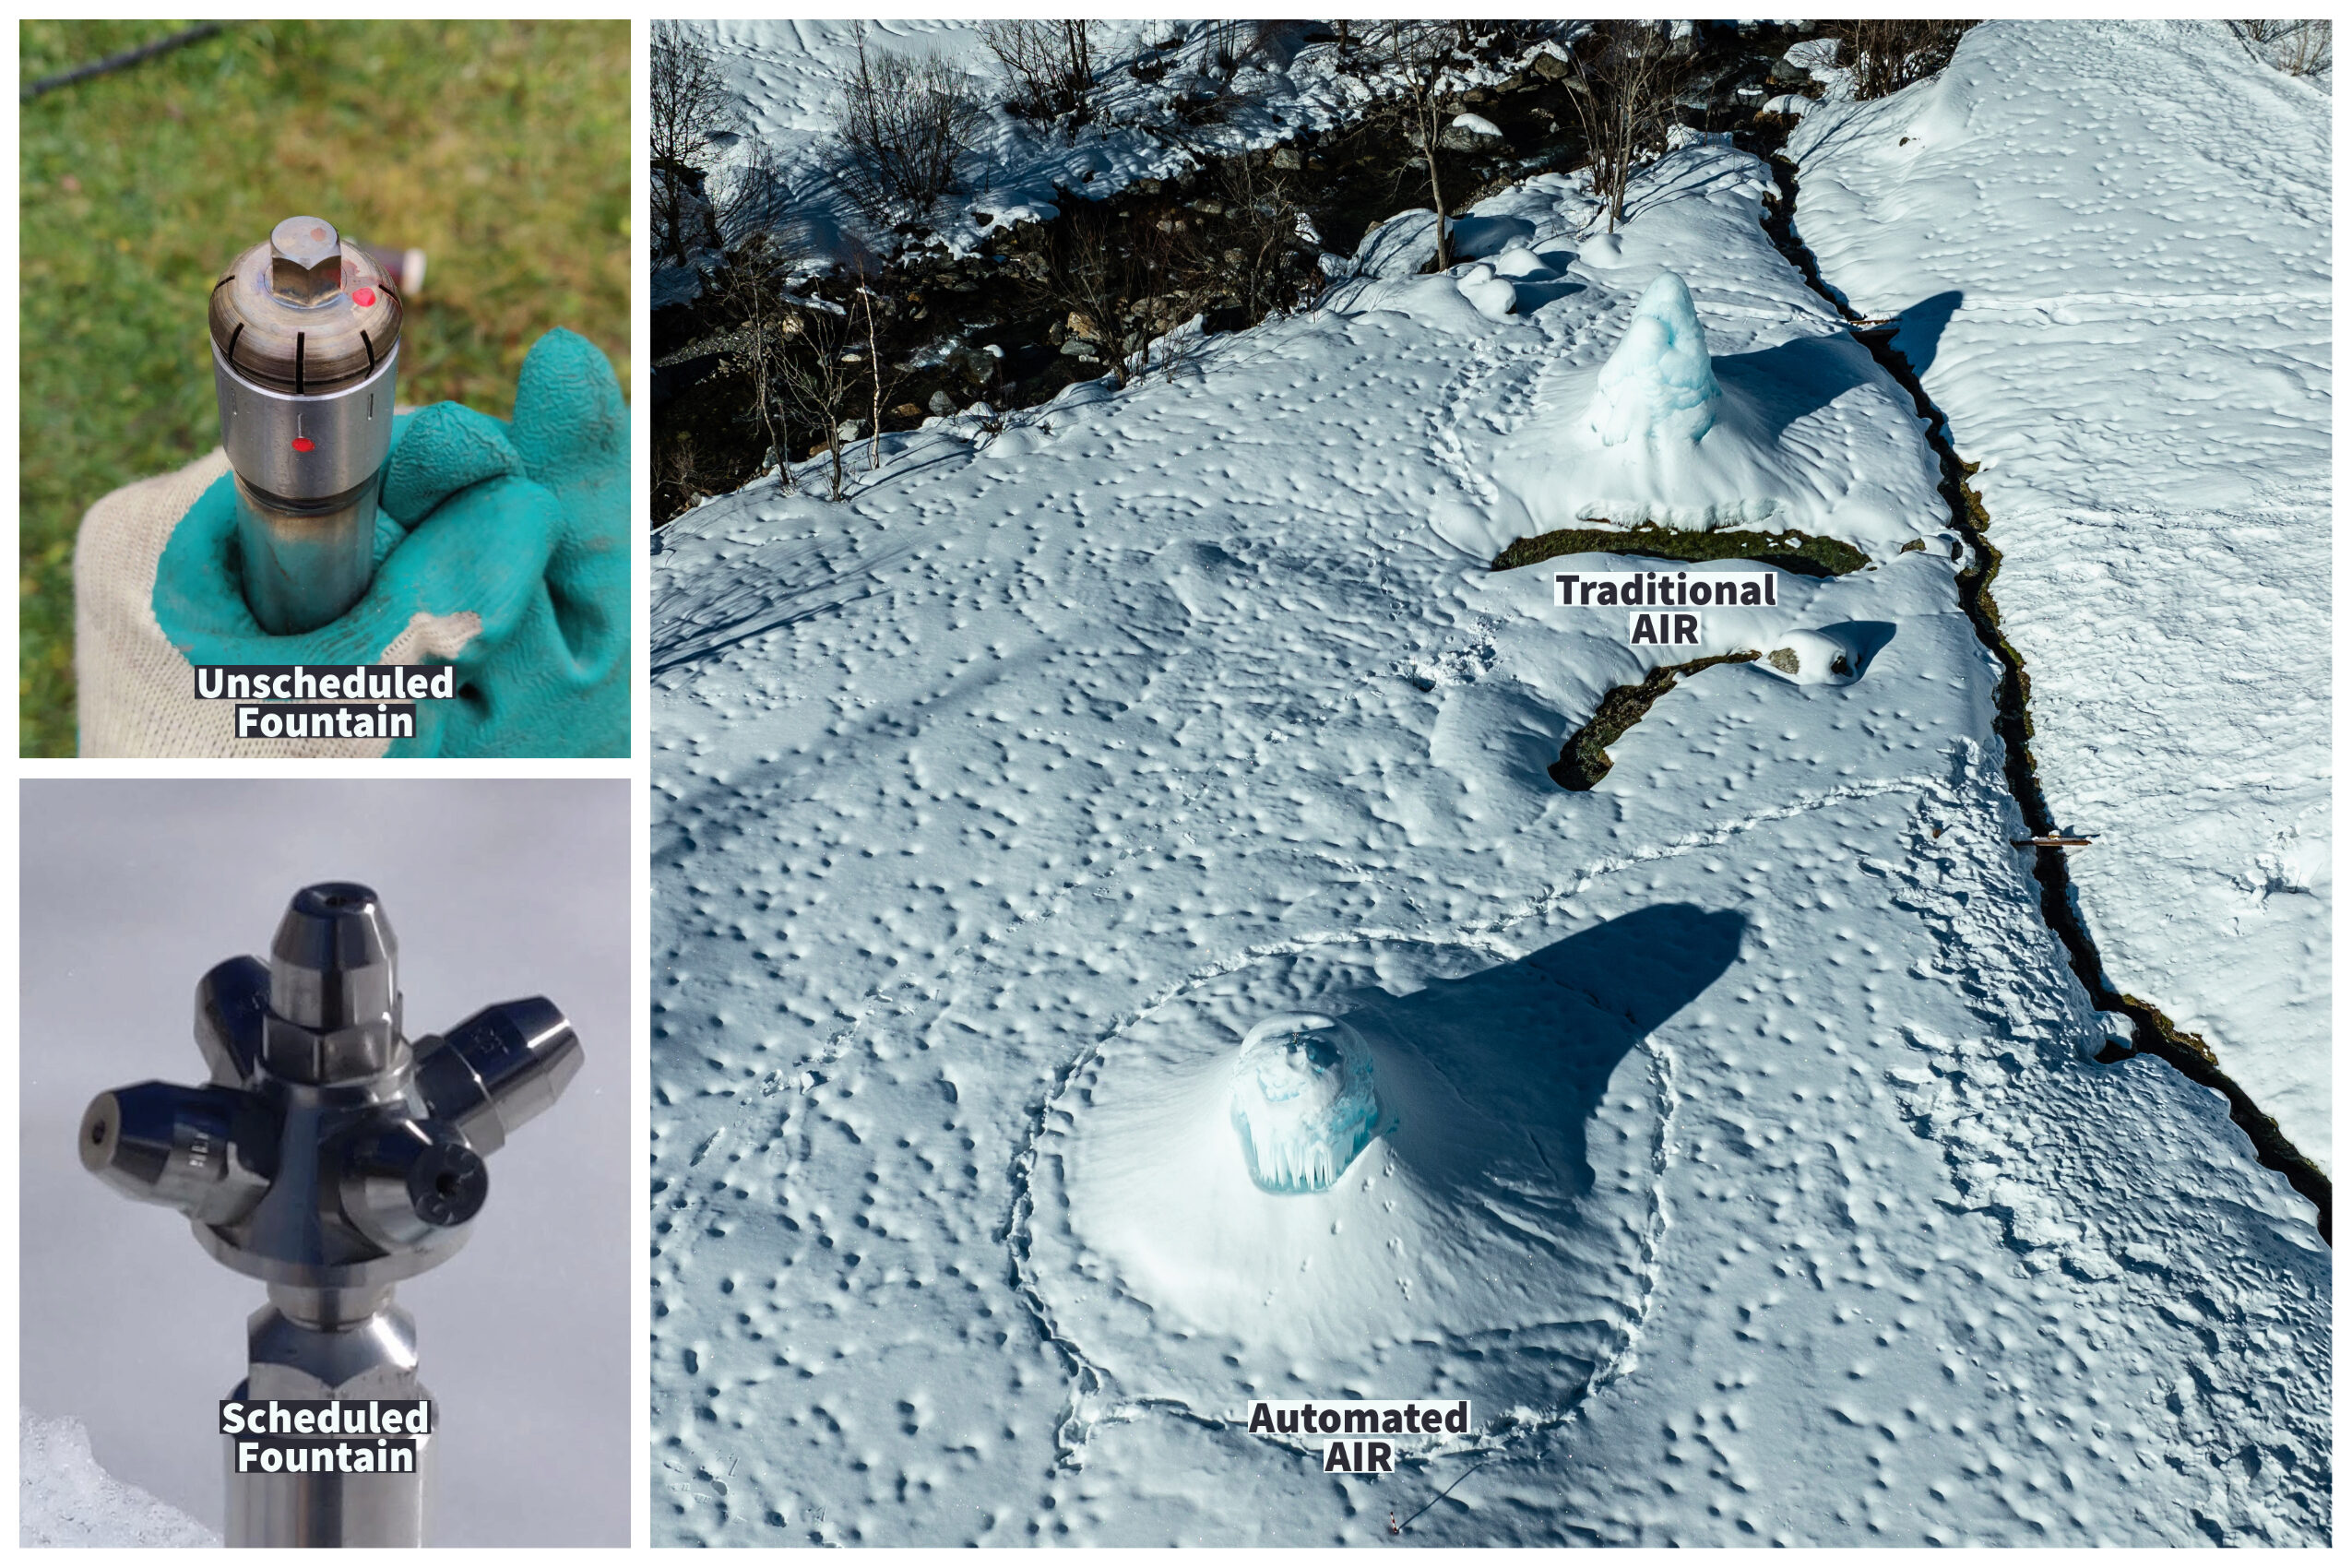
\includegraphics[width=12cm]{Figures/AIR_fountains.jpg}
\caption{Unscheduled and scheduled fountains used for construction of traditional and automated AIRs at Guttannen. Picture credits: Daniel Bürki}
\label{fig:2AIR}
\end{figure}

The automated and traditional AIRs were constructed adjacent to each other with different fountain
designs, as shown in Fig. \ref{fig:2AIR}. This ensures both AIRs share water source and identical
weather conditions. In addition, a webcam guaranteed continuous surveillance of the automated AIR.   

In the AIR constructed with the traditional strategy, tree branches were laid covering the fountain pipe to initiate and
accelerate the ice cone formation process. In the AIR constructed with an automated strategy, only the fountain pipe was placed before the
water spray started. Construction of both AIRs began on December 8, 2021 (start date) on a 13-cm-thick snow bed 
and ended on April 12, 2022 (expiry date).

In the traditional AIR, the fountain was operated manually, whereas in the automated AIR, the fountain
discharge rate was controlled using real-time weather input and several control parameters which could be
modified via a user interface. Henceforth, we refer to the fountain used in the traditional AIR as unscheduled fountain and to the fountain used in the automated
AIR as scheduled fountain.


\subsection{Meteorological data}

To calculate the surface energy balance of an AIR, the following variables are required: air temperature, relative humidity, wind speed, pressure, precipitation, incoming longwave radiation,
shortwave radiation, and cloudiness index. Our
primary weather data source is an automatic weather station (AWS) located within 20 $m$ from the AIRs. Hourly ground
temperature measurements were also recorded by the AWS to obtain approximate values of the fountain water temperature. Less
than 0.4 \% of data was missing, and data gaps were filled by linear interpolation. However,
two additional datasets were used to obtain all the necessary input variables, namely cloudiness index and
precipitation. These two datasets were obtained from ERA5 reanalysis dataset
\citep{hersbachERA5GlobalReanalysis2020} and a MeteoSwiss AWS located 184 $m$ from the AIRs (Station ID: 0-0756-0-GTT).

\begin{figure}[htb]
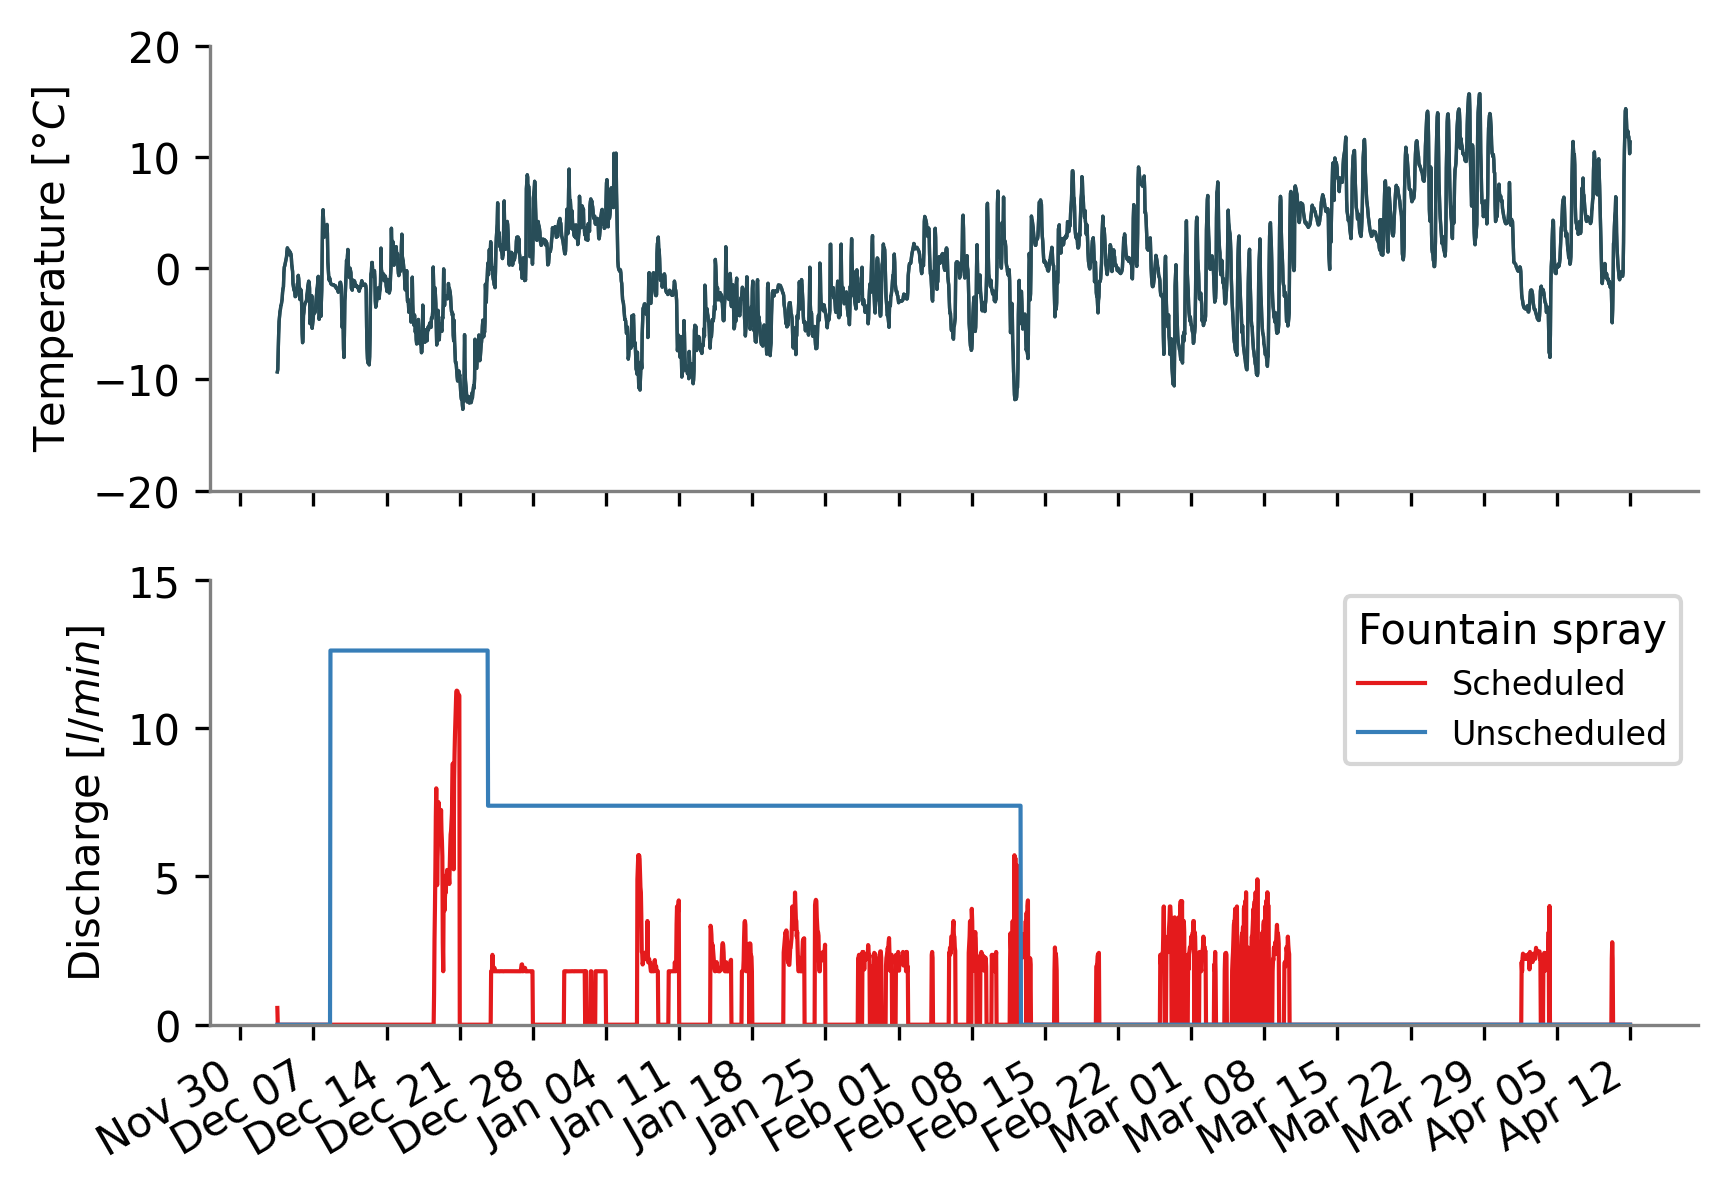
\includegraphics[width=12cm]{Figures/disvstemp.png}
\caption{Temperature and discharge measurements of the two fountains at the Guttannen construction site.}
\label{fig:aws} 
\end{figure}

\subsection{Fountain observations}

The scheduled and unscheduled fountains present the following attributes: discharge rate ($Q$), height ($h$), water
temperature ($T_F$), nozzle pressure loss ($P_{nozzle}$), and the spray radius ($r$). Discharge rate represents
the discharge rate of water in the fountain pipeline. Height denotes the height of the fountain pipeline
installed. Fountain water temperature is the temperature of water droplets produced by the fountain. The nozzle
pressure loss denotes the pressure consumed during the formation of water droplets. Spray radius denotes the
observed ice radius formed from the fountain water droplets.

Height was increased in steps of 1 $m$ for both fountains. For the scheduled fountain, the
initial height was 3 $m$ and was increased to 4 $m$ on December 23. For the unscheduled
fountain, the initial height was 3.7 $m$ and was increased twice---December
23 and February 12.

Figure \ref{fig:aws} shows the temporal variation in temperature and discharge rate for both the scheduled and
unscheduled fountains. The unscheduled fountain showed variations in discharge rate whenever the fountain height
was increased. The discharge rate variations of the scheduled fountain were caused by the control valve of the
automation system. The control ball valve position between 0 and 100 \% (or 0 to 90 $\degree$) was regulated
based on real-time meteorological conditions. Throughout the study period, the control valve was opened
completely (100 \%) only once, corresponding to the moment in time when temperature attained its minimum of $-$13
$\degree \, C$ on December 20. The control valve was never opened beyond 34 \% thereafter.  

The unscheduled fountain was manually operated to spray all the available discharge until a fountain freezing
event interrupted the discharge on February 17. Unfortunately, no discharge rate measurements were recorded
for the unscheduled fountain. However, the unscheduled fountain presented a higher discharge rate
compared with the scheduled fountain due to its higher aperture area (Fig. \ref{fig:2AIR}). Therefore, we
conservatively assume the discharge rate of the unscheduled fountain to be equal to the maximum discharge rate
of the scheduled fountain, which was observed to be 13 $l/min$ and 11 $l/min$ at a fountain height of 3 $m$ and 4
$m$, respectively.

Water temperature of both fountains was estimated from the AWS ground temperature dataset obtained with a thermistor located 0.3 $m$ below the base of the scheduled fountain.

\subsection{Drone surveys}

Several photogrammetric surveys were conducted on the traditional and the automated AIRs. The digital elevation
models (DEMs) generated from the obtained imagery were analysed to document ice radius, surface area, and
volume of the ice structures. Ice radius measurements from drone flights showed either an increase in
AIR circumference or volume and were averaged to determine the fountain spray radius. The number of drone surveys
conducted for the traditional and the automated AIRs was 8 and 6, respectively (Table \ref{tab:uav}). We
attach a high uncertainty of $\pm 10 \%$ for all AIR observations to accommodate for the uncertainties in
the drone processing methodology described in the supplementary materials of \citet{balasubramanianInfluenceMeteorologicalConditions2022}.

\begin{table}
	\centering
	\caption{Summary of drone surveys}
	\label{tab:uav}
	\begin{tabular}{@{}|llllll|@{}}
		\toprule
		\textbf{}              & \textbf{No.} & \textbf{Date} & \textbf{Volume} & \textbf{Radius} & \textbf{Surface area} \\ \midrule
		\multicolumn{1}{|l|}{\multirow{8}{*}{\rotatebox[origin=c]{90}{Traditional}}}
		                       & 1            & Dec 23, 2021  & 17 $m^{3}$     & 2.9 $m$
		                       & 47 $m^{2}$                                                                      \\
		\multicolumn{1}{|l|}{} & 2            & Jan 3, 2022  & 22 $m^{3}$     & 3.4 $m$
		                       & 61 $m^{2}$                                                                      \\
		\multicolumn{1}{|l|}{} & 3            & Jan 22, 2022   & 35 $m^{3}$     & 4 $m$
		                       & 79 $m^{2}$                                                                      \\
		\multicolumn{1}{|l|}{} & 4            & Feb 6, 2022  & 44 $m^{3}$     & 4.2 $m$
		                       & 86 $m^{2}$                                                                      \\
		\multicolumn{1}{|l|}{} & 5            & Feb 20, 2022  & 43 $m^{3}$     & 4.3 $m$
		                       & 86 $m^{2}$                                                                      \\
		\multicolumn{1}{|l|}{} & 6            & Mar 19, 2022  & 33 $m^{3}$     & 4.4 $m$
		                       & 84 $m^{2}$                                                                      \\
		\multicolumn{1}{|l|}{} & 7            & Mar 26, 2022  & 24 $m^{3}$     & 4.3 $m$
		                       & 74 $m^{2}$                                                                      \\
		\multicolumn{1}{|l|}{} & 8            & Apr 12, 2022  & 11 $m^{3}$     & 3.5 $m$
		                       & 50 $m^{2}$                                                                      
		\\\midrule
		\multicolumn{1}{|l|}{\multirow{6}{*}{\rotatebox[origin=c]{90}{Automated}}}
		                       & 1            & Dec 23, 2021  & 35 $m^{3}$      & 4.3 $m$
		                       & 73 $m^{2}$                                                                       \\
		\multicolumn{1}{|l|}{} & 2            & Jan 3, 2022   & 32 $m^{3}$      & 4.4 $m$
		                       & 81 $m^{2}$                                                                       \\
		\multicolumn{1}{|l|}{} & 3            & Feb 20, 2022   & 60 $m^{3}$      & 5.3 $m$
		                       & 105 $m^{2}$                                                                       \\
		\multicolumn{1}{|l|}{} & 4            & Mar 19, 2022   & 28 $m^{3}$      & 3.7 $m$
		                       & 57 $m^{2}$                                                                       \\
		\multicolumn{1}{|l|}{} & 5            & Mar 26, 2022   & 19 $m^{3}$      & 3.7 $m$
		                       & 53 $m^{2}$                                                                       \\
		\multicolumn{1}{|l|}{} & 6            & Apr 12, 2022   & 7 $m^{3}$      & 2.5 $m$
		                       & 53 $m^{2}$                                                                       \\
		\bottomrule
	\end{tabular}

\end{table}

\section{Methods}

\subsection{Fountain scheduling software}

Recommended discharge rates can be produced only when information about AIR surface properties and
weather conditions is available. In particular, resolving the uncertainty in the expected freezing rate requires
quantification of slope, albedo, and cloudiness. However, these properties cannot
be predicted, and therefore, we associate the upper and lower bound of each variable to a
different model depending on whether these increase the freezing rate or not. Higher albedo and slope values decrease the shortwave
radiation impact. Higher cloudiness values increase both the shortwave and the longwave radiation impact. The
model overestimating the freezing rate is hereinafter referred as ice volume optimized model (IVOM) and the model
underestimating the freezing rate, water-use efficiency optimized model (WEOM). Accordingly, the values assigned for all three variables in each model are presented in
Table \ref{tab:assumptions}.

The discharge scheduling software implements two types of fountain scheduling strategies depending on which
model type is suitable. The WEOM model type is used when the location presents limited water quantity, as this is expected to
produce better water-use efficiency. The IVOM model type is used when the location presents limited duration of favorable
weather windows, as this is expected to produce higher ice volume. These two types of scheduled fountains are hereafter referred as water-sensitive fountain and weather-sensitive fountain, respectively.

\begin{table}[htb]
\centering
\caption{Assumptions for the parametrization introduced to simplify the ice volume optimized model (IVOM) and the
water-use efficiency optimized model (WEOM). $\alpha_{snow/ice}$ represents albedo of snow or ice.}
\label{tab:assumptions}
\begin{tabular}{@{}lllll@{}}
\toprule
\textbf{Estimation of} & \textbf{Symbol} & \textbf{IVOM} & \textbf{WEOM} & \\ \midrule
\multicolumn{1}{|l}{Slope}        & $s_{cone}$ & $ 1 $ & $0$ & \multicolumn{1}{l|}{} \\ \midrule
\multicolumn{1}{|l}{Albedo} & $\alpha$ & $\alpha_{snow}$ & $\alpha_{ice}$ & \multicolumn{1}{l|}{} \\\midrule 
\multicolumn{1}{|l}{Cloudiness}  & $cld$ & $0$ & $1$ & \multicolumn{1}{l|}{} \\ \bottomrule
\end{tabular}
\end{table}

We apply the assumptions described in Table \ref{tab:assumptions} on the one-dimensional description of energy
fluxes as used in \cite{balasubramanianInfluenceMeteorologicalConditions2022} to obtain the rate of change of
AIR ice mass as follows: 

\begin{equation}
  \frac{\Delta M_{ice}}{\Delta t}  =  (\frac{q_{SW} + q_{LW} + q_{S} + q_{F} + q_{R} + q_{G} - q_{T}}{L_F} + \frac{q_{L}}{L_V} ) \cdot A_{cone}
	\label{eqn:auto}
\end{equation}

Upward and downward fluxes relative to the ice surface are positive and negative, respectively. The first term
represents the mass change rate due to freezing of the fountain water and melting of the ice. $q_{SW}$ is the
net shortwave radiation; $q_{LW}$ is the net longwave radiation; $q_{L}$ and $q_{S}$ are the turbulent latent
and sensible heat fluxes, respectively; $q_{F}$ is the fountain discharge heat flux; $q_{R}$ is the rain water heat flux;
$q_{G}$ is the ground heat flux; $q_{T}$ is the temperature heat flux, and $A_{cone}$ is the area of the AIR
surface. $L_F$ and $L_{V}$ represent latent heat of fusion and vaporization, respectively. The derivation of
these individual terms for the IVOM and WEOM model versions are discussed in Appendix \ref{sec:SEB}.

Equation \ref{eqn:auto} is implemented in the automation software. The user interface of the software enables
input of the spray radius, altitude, latitude, and longitude of the construction location. The automation
hardware consists of an AWS, flowmeter, control valve, drain valves, air valves, fountain, pipeline, and a
logger. The logger feeds the AWS data to the automation software and informs of the recommended discharge rate to
the flowmeter. The flowmeter adjusts the control valve to match the recommendation. In case a termination
criterion gets met, the drain and air valves allow removal of water and entry of
air in the pipeline, respectively.

The recommended discharge rate is equal to the mass change rate. However, certain termination criteria listed
below override the discharge rate recommendation and drain the pipeline to prevent water loss or fountain
freezing events:

\begin{itemize}

\item High water loss is assumed when wind speed is greater than user-defined critical wind speed.

\item High risk of fountain freezing is assumed when mass change rate is lower than user-defined minimum fountain discharge rate. 

\item Freezing events in fountain pipeline are assumed when measured discharge rate equals zero for at least 20
  seconds. 

\item Pipeline leakage is assumed when measured discharge rate is greater than user-defined maximum fountain discharge rate.

\end{itemize}

\section{Modelling fountain spray radius} \label{sec:r_F}

Fountain spray radius is defined as the largest horizontal distance covered by fountain water droplets. This
can be determined by modelling the trajectory of these droplets using the projectile motion equation. This
projectile motion starts at the fountain nozzle and ends at the AIR surface.  To obtain the droplets speed
($v$), we use the measured aperture diameter ($dia = 0.001 m$) and discharge rate of the scheduled fountain
with the following equation:

\begin{equation}
	\label{eqn:dis}
v = \frac{4 \cdot Q}{60 \cdot 1000 \cdot \pi \cdot dia^2}
\end{equation}

where $v$ is the droplet speed in $m/s$ and $Q$ is the discharge rate of the fountain in $l/min$.

To obtain the spray radius ($r$), we use the optimum launch angle $\theta = 45 \degree$ in the projectile motion
equation to get:

\begin{equation}
  \label{eqn:radf}
  r = \frac{v \cdot(v + \sqrt{v^2 + 4hg)}}{2g}
\end{equation}

The influence of wind-driven redistribution can be included in the spray radius by multiplying wind speed
by time of flight of water droplets.

\section{Determination of pressure losses} \label{sec:p_loss}

The fountain pipeline system delivering water to the ice stupa suffers several pressure losses, which
limit the maximum height that the fountain can achieve. These lossses can be (a)
altitudinal ($P_{alt}$), (b) frictional ($P_{friction}$), and (c) nozzle ($P_{nozzle}$) losses. The altitudinal
losses depend on the altitude difference between the source and the fountain. The frictional losses are
proportional to the length of the pipeline and inversely proportional to their diameter. The nozzle losses
depend on the engineering design of the fountain nozzle.

Pressure losses can be determined using the Bernoulli equation as follows:

\begin{equation}
  \label{eqn:pressure}
  P_{source} = P_{alt} + P_{friction} + P_{nozzle} + \frac{\rho \cdot v^2}{2} \cdot 10 ^{-5}
\end{equation}

where $P_{source}$ is the source pressure, $P_{nozzle}$ is the pressure loss due to the fountain nozzle, and
$P_{alt}$ is the pressure loss due to the altitudinal difference between the pipeline input and fountain output. These pressure variables are measured in bars.  The speed $v$ can be determined from discharge rate
observations using Eq. \ref{eqn:dis}. 

The frictional loss of the pipeline used in the experiment can be determined using the 
Hagen–Poiseuille equation \citep{poiseuilleExperimentalInvestigationsFlow1847}:  

\begin{equation}
  \label{eqn:friction}
  P_{friction} = \frac{3.2 \cdot \mu \cdot v \cdot L}{\rho \cdot g \cdot dia^2}
\end{equation}

where $P_{friction}$ is in bars, $L$ is the total length of the pipeline measured in meters, and $v$ is the water speed in
$m/s$. Note that the above equation only applies for laminar flow, the one investigated in the present work.


\subsection{Model updates}

In the present study, we focus on the
integration of fountain scheduling processes with the AIR model
\citep{balasubramanianInfluenceMeteorologicalConditions2022}. For details on model internals and 
calculation of surface processes, we refer to the respective literature references. 

In the previous version of the model \citep{balasubramanianInfluenceMeteorologicalConditions2022}, fountain
water temperature ($T_F$) was estimated as a constant parameter. However, in reality, this is a poor
approximation because it does not account for two processes, namely temperature fluctuations during transit
from the source to the fountain nozzle or temperature fluctuations during the flight time of water
droplets after leaving the fountain nozzle. Therefore, we use hourly measured ground temperature
values to approximate the first process and we assume that water temperature cools down to 0 $\degree\,C$ during subzero
air temperature conditions to approximate the second process.

In the previous version of the model \citep{balasubramanianInfluenceMeteorologicalConditions2022}, fountain
discharge events were reset from surface albedo to ice albedo. However, this assumption limits the accuracy of
the model, especially for the automated AIR, where several fountain discharge events of short duration occur.
Therefore, we assume that discharge events reduce the albedo decay rate ($\tau$) by a 
factor of $\frac{\alpha_{ice}}{\alpha_{snow}}$.

Additionally, both AIRs experienced numerous precipitation events. Therefore, instead of 
assuming AIR density ($\rho_{cone}$) to be equal to ice density---which was no longer accurate---we parameterized AIR density $\rho_{cone}$ as follows:

\begin{equation}
  \rho_{cone} = \frac{M_{F} + M_{dep} + M_{ppt}}{(M_{F} + M_{dep})/\rho_{ice} + M_{ppt}/\rho_{snow}}
\end{equation}

where $M_F$ is the cumulative mass of the fountain discharge, $M_{ppt}$ is the cumulative precipitation,
$M_{dep}$ is the cumulative accumulation through water vapour deposition, $\rho_{ice}$ is the ice density (917
$kg\,m^{-3}$), and $\rho_{snow}$ is the density of wet snow (300 $kg\,m^{-3}$) taken from
\cite{cuffeyPhysicsGlaciers2010}.

Rain events were not considered in the previous version of the model, but these occurred in our experiment. The
influence of rain events on the albedo and the energy balance was assumed to be similar to the discharge events.
However, the water temperature of a rain event was assumed to be equal to the air temperature; accordingly, the
rain water heat flux ($q_{R}$) generated due to a rain event was equal to:

\begin{equation}
  q_{R} = \frac{\Delta M_{ppt} \cdot c_{water} \cdot T_{a}}{\Delta t \cdot A_{cone}}
\end{equation}

where $M_{ppt}$ is the hourly precipitation in meters, $c_{water}$ is the specific heat of water, and $A_{cone}$
is the surface area.

\subsection{Calibration}

The model parameters were calibrated to the mean values of the ranges presented in Appendix Table
\ref{tab:parameters}. However, the surface layer thickness parameter was calibrated to a value of 0.09 $m$ for the
automated AIR instead of the default value of 0.05 $m$. This calibration was necessary to prevent hourly surface
temperature fluctuations from assuming unphysical values above 40 $\degree\,C$.

We performed the validation of the model for the traditional and automated AIRs by evaluating the root mean
squared error (RMSE) between volume estimates and measurements. 

Performance of the IVOM and WEOM versions of the physical model were assessed by comparing the correlation of its
discharge rate estimates with the validated freezing rates of the traditional AIR.

\section{Results}

\subsection{Model validation}

The volume estimation for the automated and traditional AIRs showed an RMSE of 8 $m^3$ and 6 $m^3$, respectively, with the drone
volume observations. These are within 13 \% and 11 \% of the maximum volume of the automated and
the traditional AIR, respectively. The estimated and measured AIR volumes are shown in Fig. \ref{fig:validation}.  

\begin{figure}[htb] 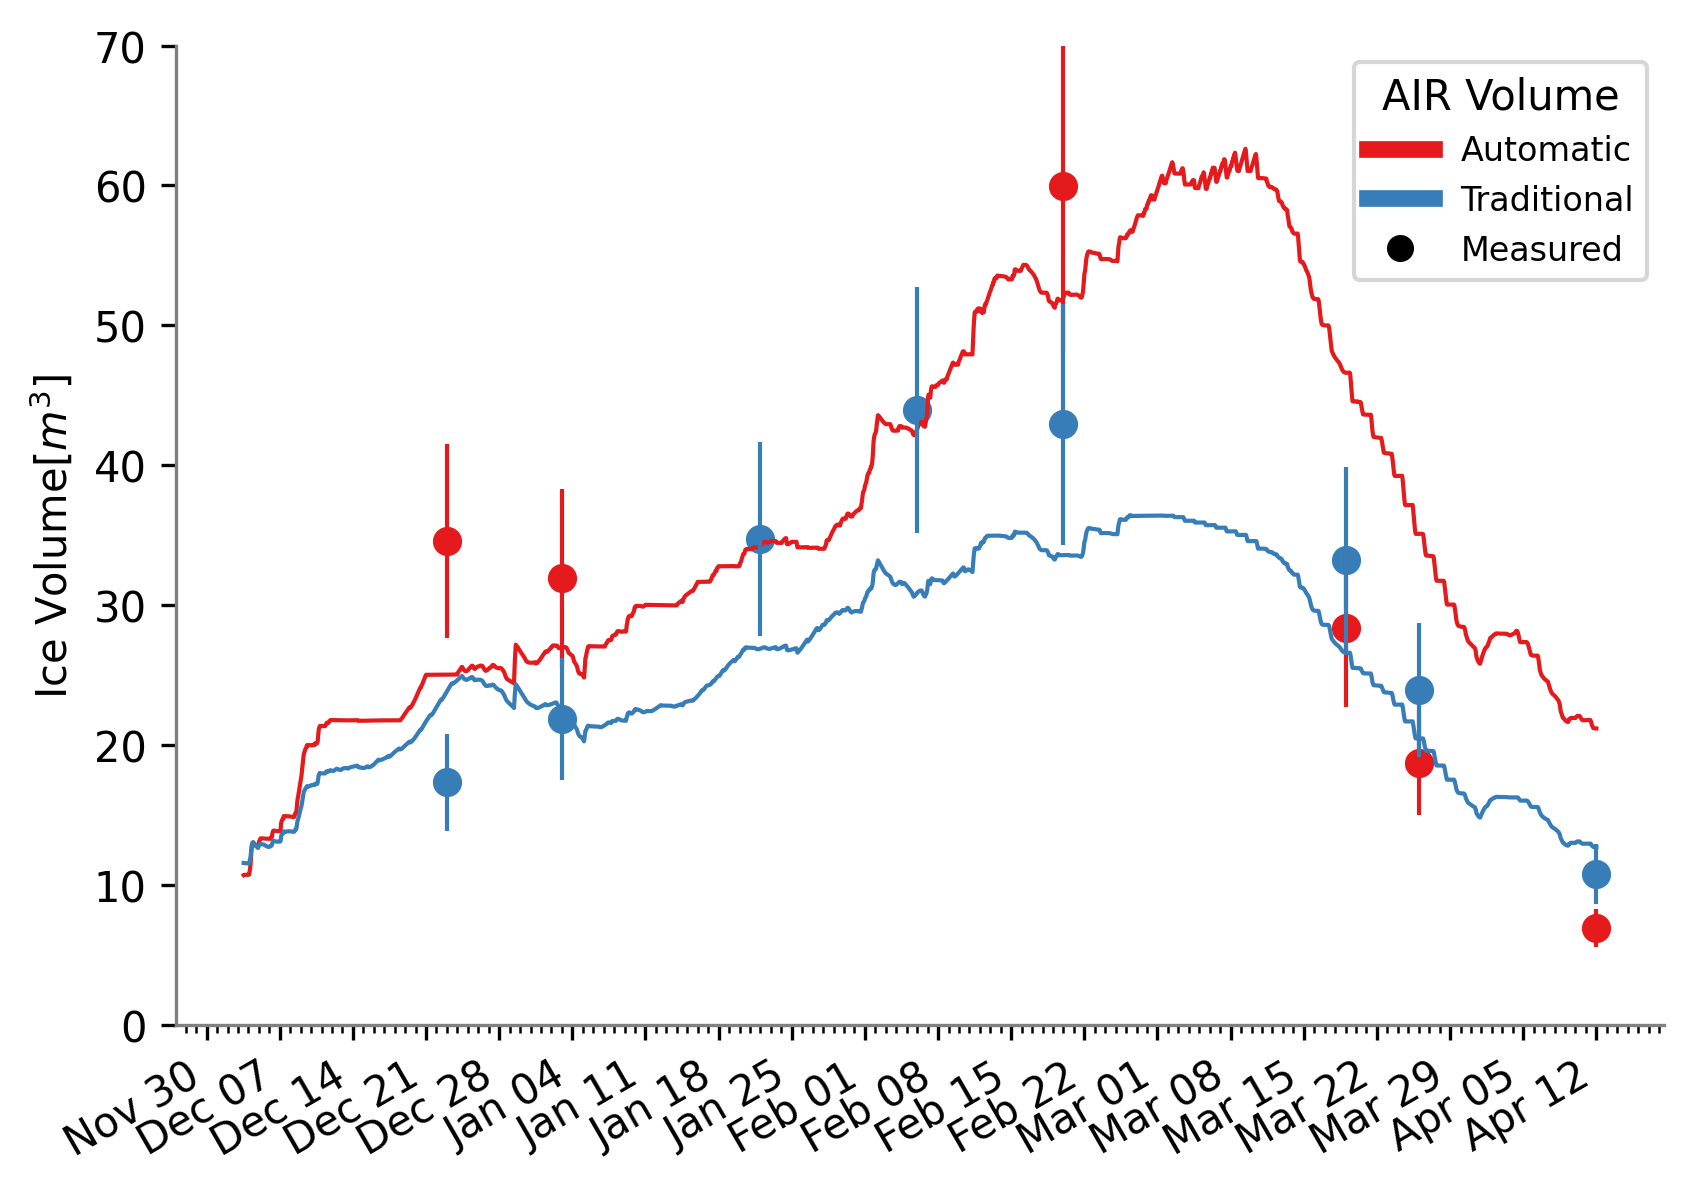
\includegraphics[width=12cm] {Figures/validation.png} 
  \caption{Volume validation of the scheduled and unscheduled fountain construction strategies.} 
  \label{fig:validation} \end{figure}


\begin{table}
	\centering
	\caption{Summary of the mass balance, energy balance, and fountain and AIR characteristics estimated at the end of the respective
  simulation duration for the automated and the traditional AIRs}
	\label{tab:mb}
	\begin{tabular}{@{}|llllll|@{}}
		\toprule
		\textbf{}              & \textbf{Name}                   & \textbf{Symbol} & \textbf{Traditional} & \textbf{Automated} &
		\textbf{Units}                                                                                                       \\ \midrule
		\multicolumn{1}{|l|}{\multirow{3}{*}{\rotatebox[origin=c]{90}{Input}}}
		                       & Fountain discharge              & $M_F$           & \num{1.1e6}   & \num{1.5e5}     & $kg$  \\
		\multicolumn{1}{|l|}{} & Snowfall                        & $M_{ppt}$       & \num{9.2e3}   & \num{1.4e4}   & $kg$  \\
		\multicolumn{1}{|l|}{} & Deposition                      & $M_{dep}$       & \num{4.0e2}   & \num{4.5e2}     & $kg$  \\ \midrule
		\multicolumn{1}{|l|}{\multirow{4}{*}{\rotatebox[origin=c]{90}{Output}}}
		                       & Meltwater                       & $M_{water}$     & \num{4.5e4} & \num{5.4e4}   & $kg$  \\
		\multicolumn{1}{|l|}{} & Ice                             & $M_{ice}$       & \num{7.4e3} & \num{6.1e3}    & $kg$  \\
		\multicolumn{1}{|l|}{} & Sublimation                     & $M_{sub}$       & \num{3.7e3} & \num{4.5e3}     & $kg$  \\
		\multicolumn{1}{|l|}{} & Fountain wastewater             & $M_{waste}$     & \num{1.07e6} & \num{1.0e5}     & $kg$  \\ \midrule
		\multicolumn{1}{|l|}{\multirow{7}{*}{\rotatebox[origin=c]{90}{Energy flux}}}
                           & Shortwave radiation             &  $q_{SW}$       & $14$  & $21$ & \% \\
		\multicolumn{1}{|l|}{} & Longwave radiation              &  $q_{LW}$       & $25$  & $25$ & \% \\
		\multicolumn{1}{|l|}{} & Sensible heat                   &  $q_{S}$        & $38$   & $33$ & \% \\
		\multicolumn{1}{|l|}{} & Latent heat                     &  $q_{L}$        & $19$  & $19$ & \% \\
		\multicolumn{1}{|l|}{} & Fountain discharge heat         &  $q_{F}$        & $4$  & $0$     & \% \\
		\multicolumn{1}{|l|}{} & Rain heat                       &  $q_{R}$        & $0$  & $0$     & \% \\
		\multicolumn{1}{|l|}{} & Ground heat                     &  $q_{G}$        & $1$   & $1$     & \% \\\midrule
		\multicolumn{1}{|l|}{\multirow{2}{*}{\rotatebox[origin=c]{90}{AIR}}}

		                       & Maximum AIR volume              &                 & 53            & 61            & $m^{3}$ \\
		\multicolumn{1}{|l|}{} & Water-use efficiency            &                 & 4             & 35            & \% \\\midrule
	\end{tabular}
\end{table}

\subsection{Comparison of AIR construction strategies}

Table \ref{tab:mb} presents the influence of the two different fountain scheduling strategies in the mass and energy balance
of their respective AIRs.  The overall impact of the radiation fluxes---longwave and shortwave---and the
turbulent fluxes---sensible and latent---on the freezing and melting energies is determined by their 
energy turnover, which is calculated as the sum of energy fluxes in absolute values (Table
\ref{tab:mb}). 

\begin{figure}[htb]
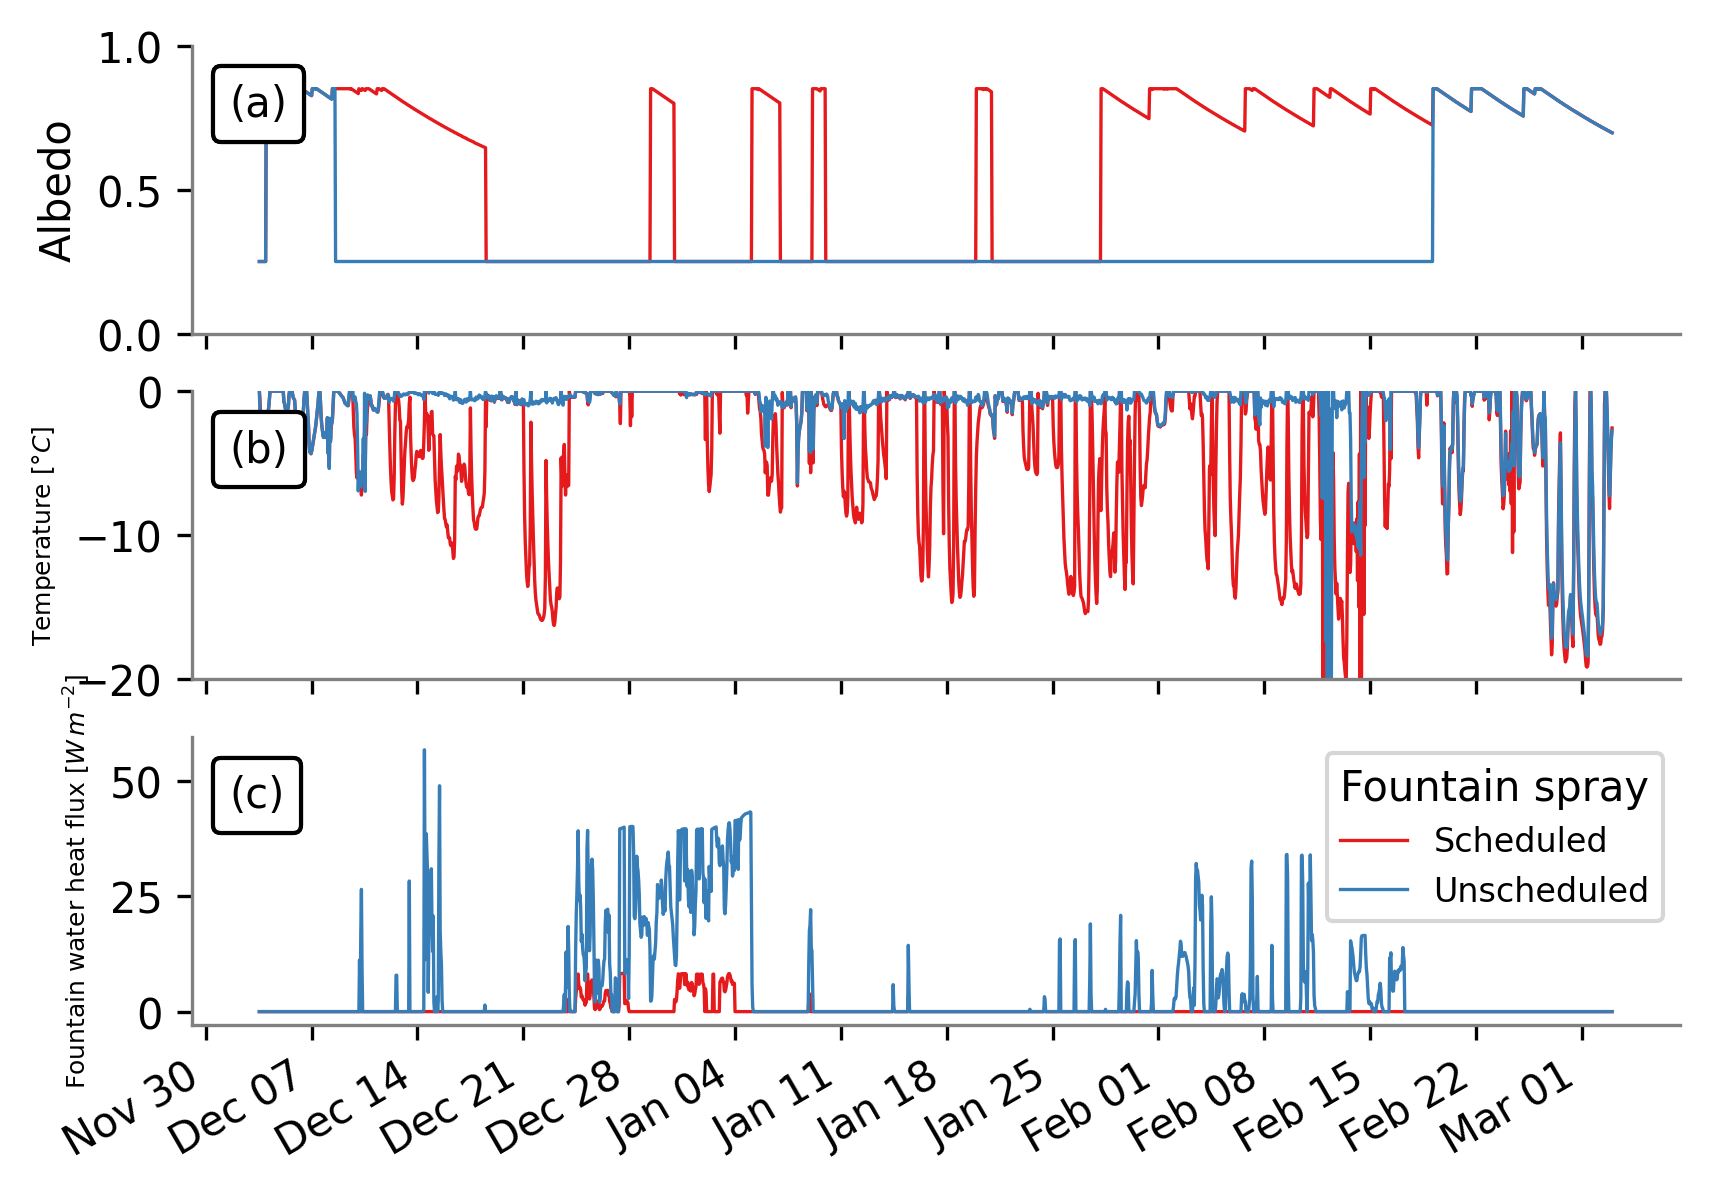
\includegraphics[width=12cm]{Figures/dis_processes.png}
\caption{(a) Surface albedo  and (b) fountain discharge heat flux showed significant variations between the two
  AIRs due to differences in their discharge rates.}
\label{fig:dis_processes}
\end{figure}

Fountain scheduling reduced the fountain discharge input and fountain wastewater output by an order of
magnitude. However, this does not result in an appreciable difference in the volume evolution of the automated
or traditional AIR, as shown in Fig. \ref{fig:validation}. This is due to two counteracting surface processes
during fountain spray: process A consists in the dampening of albedo to ice albedo and process B consists in the absorption of heat energy from the
fountain water droplets. The temporal variation of the magnitude of these processes is shown in Fig.
\ref{fig:dis_processes}.

A considerable difference exists in the contribution of the shortwave radiation due to process A. Although the unscheduled fountain was active for a longer duration, frequent snowfall events
counteracted the albedo feedback of the fountain discharge. In contrast, the albedo of the automated AIR was
reduced by late fountain spray events, in particular in March and April, as shown in Fig.
\ref{fig:dis_processes}. These poorly timed fountain spray events occurred because of the global solar radiation
diurnal variation, since these were calibrated based on values for February in the automation system.
Therefore, poor calibration of the automation system resulted in an increased impact of shortwave radiation on
the automated AIR. Similarly, the fountain discharge heat flux for the traditional AIR was enhanced due to
process B. The higher discharge value of the unscheduled fountain and its longer duration are responsible
for the higher contribution of fountain discharge heat flux in the overall energy turnover. Therefore, higher
melt of the automated AIR due to process A counteracted the higher melt of the traditional AIR due to process B.

\subsection{Benefits of scheduling fountains}

The difference in water-use efficiency and maximum ice volume between unscheduled and scheduled fountains in the Indian and Swiss
locations across two winters is shown in Fig. \ref{fig:wue}a. Four experimental values (highlighted in
circles) and five simulated values (highlighted in squares) are shown together.  The experimental values were
taken from the IN21 and CH21 AIRs studied in \citet{balasubramanianInfluenceMeteorologicalConditions2022} and
the CH22 AIR investigated in the present work. 

\begin{figure*}[htb]
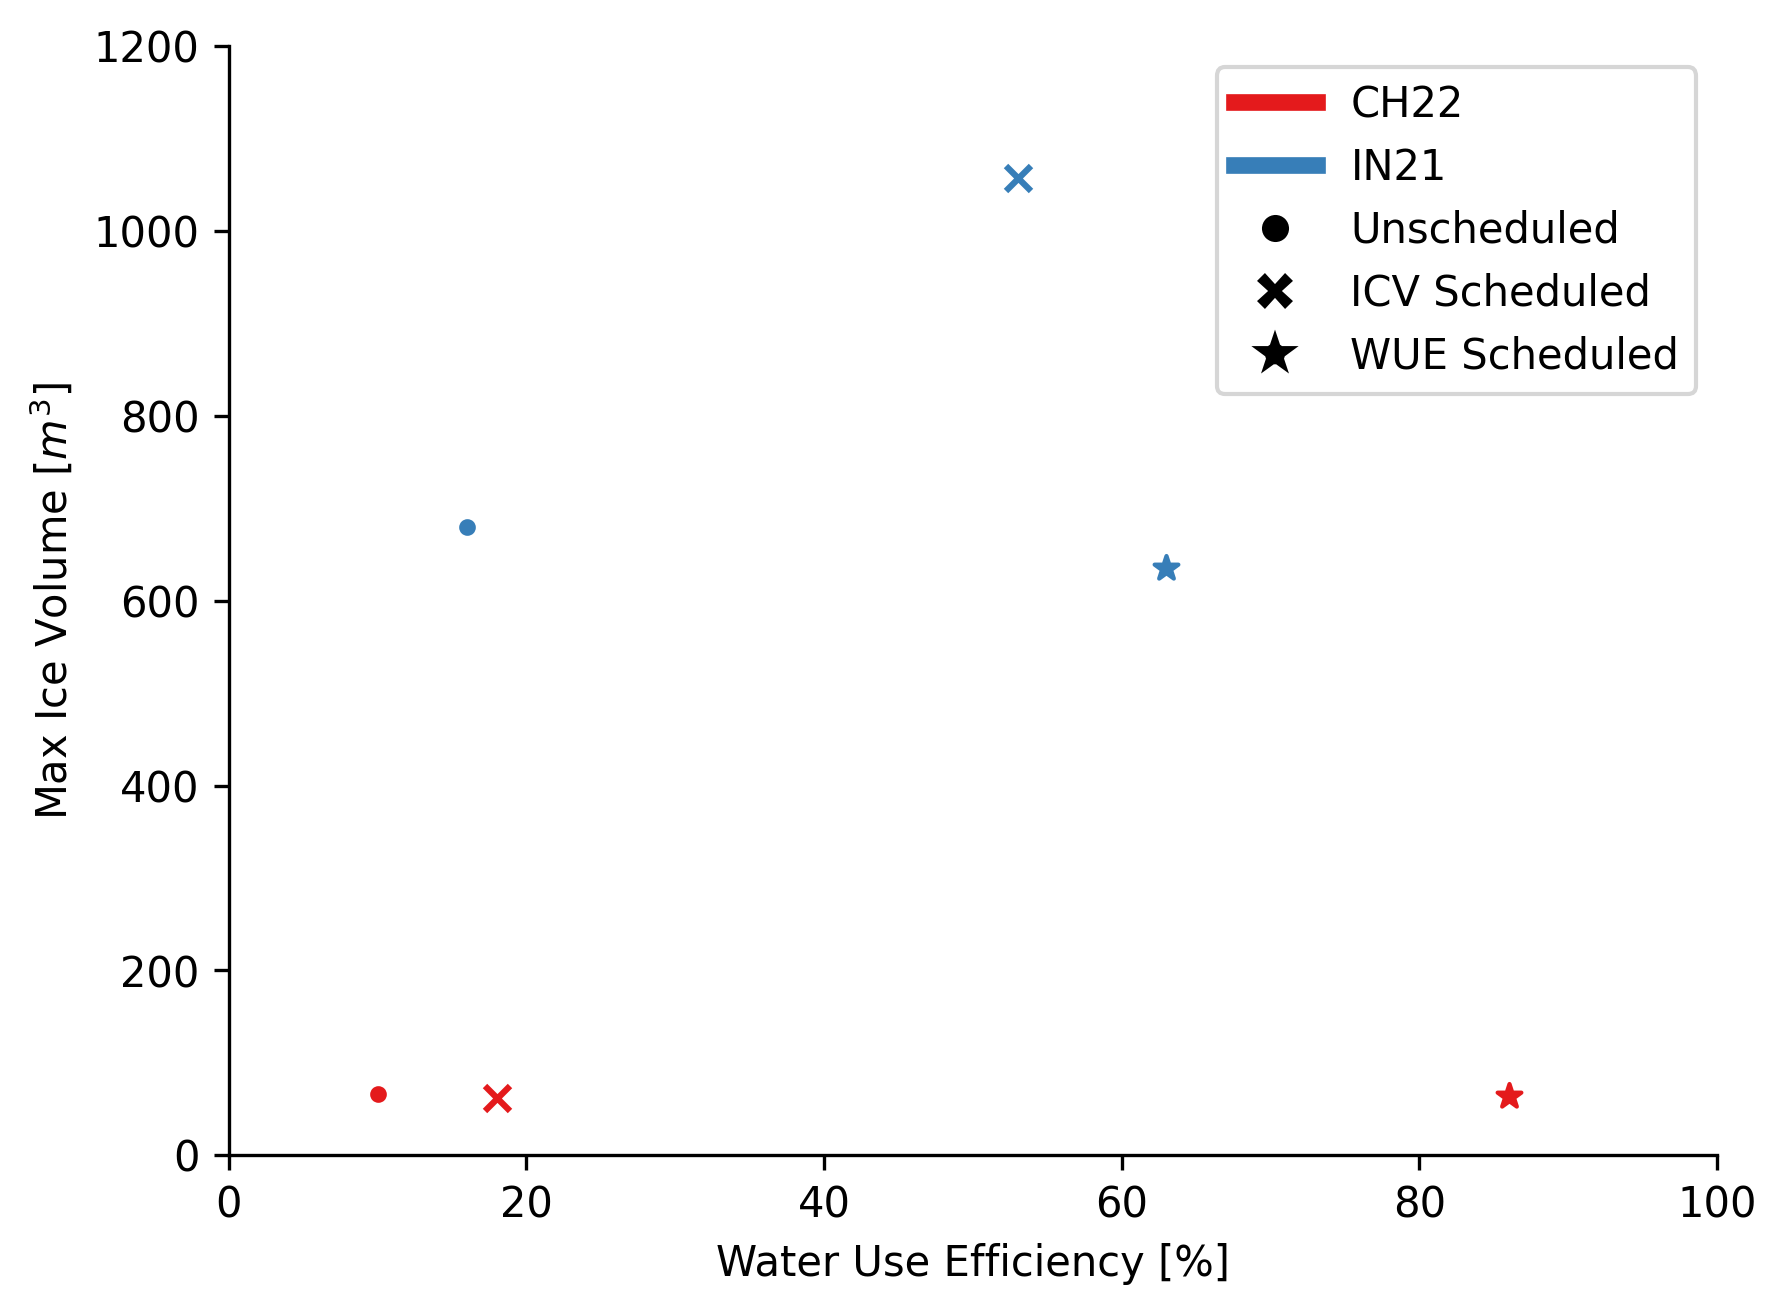
\includegraphics[width=\textwidth]{Figures/wue.png}

\caption{(a) The maximum volume and water-use efficiency estimated for AIRs constructed in different locations
(represented by symbols) with different fountain scheduling strategies (represented by colours). Experimental
values are highlighted in circles and simulated values are highlighted in squares. (b) Comparison of
the unscheduled and scheduled fountain discharge rates at the IN21 location.}

\label{fig:wue}
\end{figure*}

The water-use efficiency of all the unscheduled fountains is below 20 \%. In general, water-use efficiency
exhibits a threefold increase when the weather- or water-sensitive fountains are used in both
locations.  

For the Indian location, the three different kinds of fountains yielded significantly different results owing to discharge
duration and max discharge rate
(Fig. \ref{fig:wue}b). The unscheduled fountain showed a max discharge rate more than twice that of
the scheduled fountains, resulting in higher water loss; freezing events in its pipeline caused frequent
interruptions in the unscheduled discharge rate (Fig. \ref{fig:wue}b). In contrast, the mean freezing
rates of the other two fountains during these events were above their median values. This is because very cold
temperatures freeze the water inside rather than outside the fountain system, instigating these freezing events in
the fountain pipeline. Therefore, the discharge duration of the unscheduled fountain was much lower, resulting in
lower ice volume. The water-sensitive fountain underestimated the freezing rate during the construction period
and therefore produced much lower ice volume compared with the weather-sensitive fountain. 

For the Swiss locations, scheduled fountains yielded better water-use efficiency but did not significantly alter the maximum
volume obtained. 

\subsection{Performance of weather- and water-sensitive fountains}

The WEOM and IVOM model versions estimated the
freezing rate of the unscheduled fountain with an RMSE less than 0.8 $l/min$ and 1.8
$l/min$, respectively, and a correlation of 0.4. The discharge rate values of the weather-sensitive fountain overestimated the freezing
rate 93 \% of the fountain spray duration, whereas those of the water-sensitive fountain overestimated the
freezing rate 70 \% of the unscheduled fountain spray duration, as illustrated by Fig. \ref{fig:simvsreal}.
Therefore, the IVOM model version was successful in prioritizing the maximum ice volume by overestimating the
discharge rates, but the WEOM model version could not sufficiently underestimate its discharge rate values to
optimize water-use efficiency.

\begin{figure*}[htb]
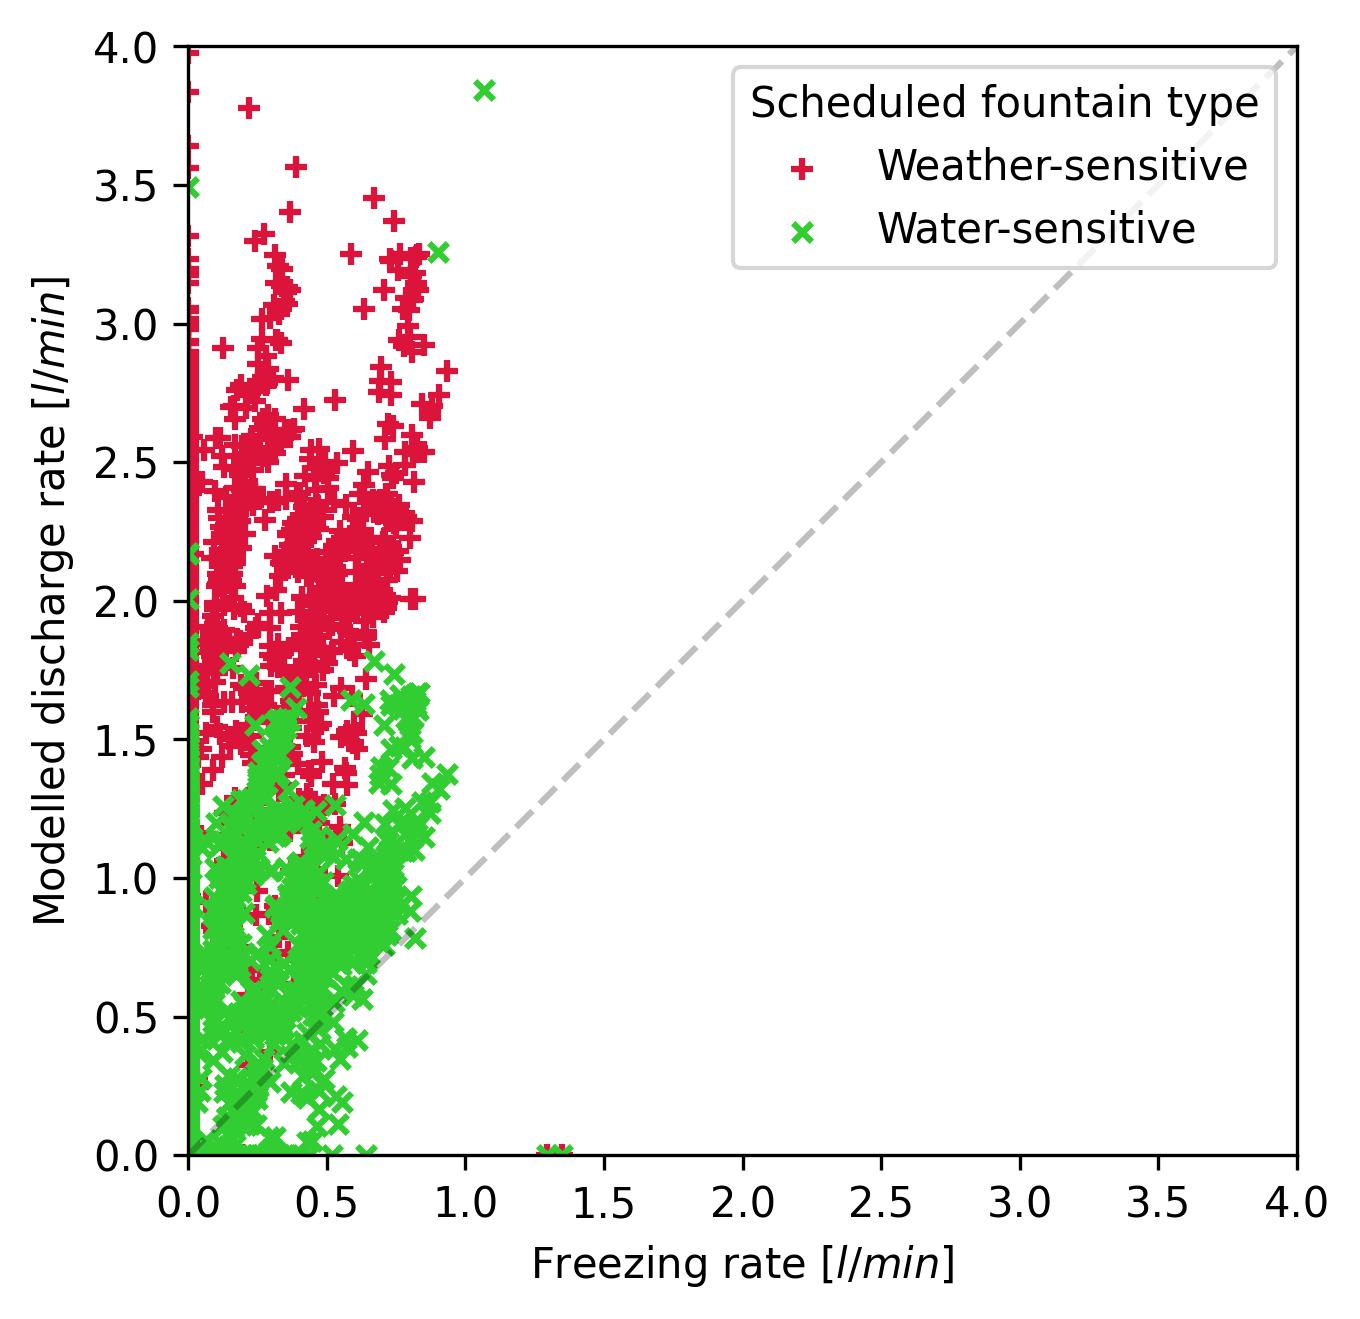
\includegraphics[width=8cm]{Figures/simvsreal.jpg}

\caption{ Comparison of the freezing rate estimated for the unscheduled fountain and the discharge rate of the
scheduled fountains. }

\label{fig:simvsreal}
\end{figure*}

However, for the Indian location, significant magnitude differences can be observed among the three kinds of
fountains. The modelled weather- and water-sensitive discharge rate values were a factor of two and three smaller, respectively,
than the measured unscheduled discharge rate (Fig. \ref{fig:wue}b).


\subsection{Pressure losses}

\begin{table}[htb]
\centering
\caption{Pipeline configuration of the automated ice stupa.}
\label{tab:pipe}
\begin{tabular}{@{}llll@{}}
\toprule
\textbf{Name} & \textbf{Symbol} & \textbf{Value} & \\ \midrule
\multicolumn{1}{|l}{Pipeline diameter}      & $dia$ & 16 $mm$ & \multicolumn{1}{l|}{} \\ \midrule
\multicolumn{1}{|l}{Pipeline length}        & $L$ & 66 $m$ & \multicolumn{1}{l|}{} \\ \midrule
\multicolumn{1}{|l}{Source water pressure} & $P_{source}$ & 6 $bar$  & \multicolumn{1}{l|}{} \\\midrule 
\multicolumn{1}{|l}{Altitudinal pressure head}  & $P_{alt}$ & 1.1 $bar$ & \multicolumn{1}{l|}{} \\ \midrule
\multicolumn{1}{|l}{Water viscosity}  & $\mu$ & 0.00152 $Pa\,s$ & \multicolumn{1}{l|}{} \\ \bottomrule
\end{tabular}
\end{table}

Pressure consumption across the fountain pipeline provides insights into how the fountain pipeline
configuration can be better optimized. The pipeline configuration of the automated ice stupa fountain is presented
in Table \ref{tab:pipe}. Maximum frictional loss occurs during maximum discharge, which was measured to be 11
$l/min$. By substituting the corresponding values in Eq. \ref{eqn:friction}, we get $P_{friction}$ to be 0.3
$bar$. The speed $v$ can be determined from our discharge rate observation from Eq. \ref{eqn:radf}.
Therefore, from Eq. \ref{eqn:pressure}, we get $P_{nozzle}$ to be 4.6 $bar$, which represents more than 75 \% of the
source water pressure. Most of the input pressure was used by the fountain nozzle to generate water droplets.

\subsection{Influence of wind-driven redistribution on fountain spray radius}

The estimated volume changes over the month of January of the Swiss AIRs built in the winter of 2021--22 is less
than half that of the AIRs from the previous winter (CH21). This difference cannot respond to warmer
temperatures during the CH22 winter, as the median January temperature of CH22 winter was colder than that of the
CH21 winter (Fig. \ref{fig:CH_diffs}a). Moreover, the volume growth of CH20 AIR is 6 times that of the CH22 AIR,
despite CH20 winter being 3 $\degree C$ warmer.

We suspect the primary driver of volume difference across different winters to be the spray radius (Fig. \ref{fig:CH_diffs}b). However, this observation contradicts our expectation that AIRs using the same
water source and fountain designs would present similar spray radius. Moreover, manual measurements of the fountain spray
radius were lower than the drone observations of the ice radius. These two observations imply
that wind drift of water droplets could play a major role in temporal fluctuations of ice radius.

\begin{figure*}[htb]
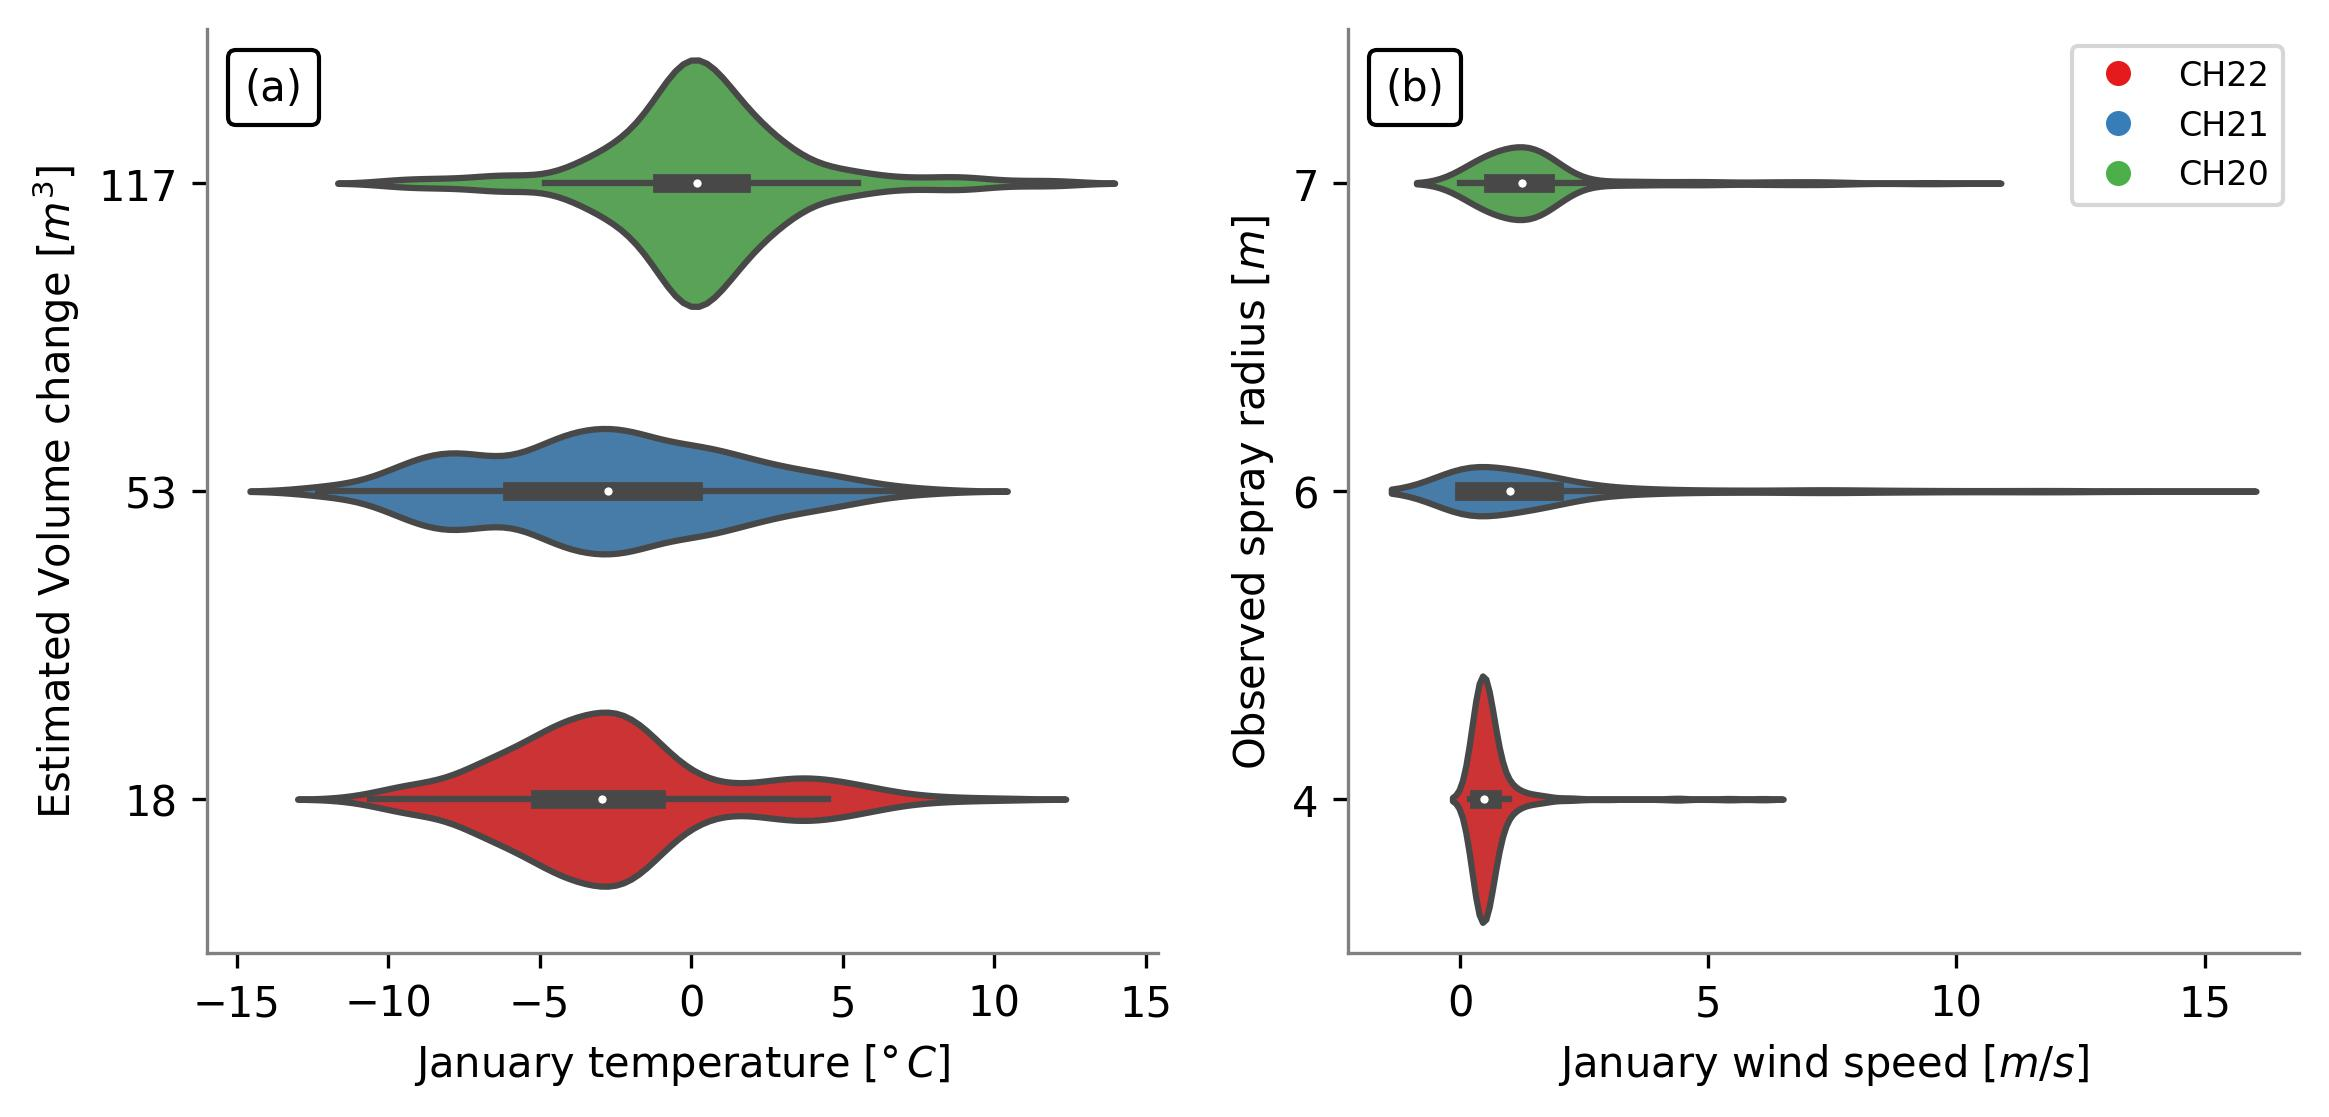
\includegraphics[width=\textwidth]{Figures/CH_diffs.jpg}

\caption{(a) Estimated volume change and temperature. (b) Observed spray radius and wind speed
during January for AIRs built across three winters. } 

\label{fig:CH_diffs} 
\end{figure*}

To validate this hypothesis, we modelled the projectile motion of scheduled fountain water droplets with wind speed
values taken from CH22 and CH21 experiments. Figure \ref{fig:wind} shows the modelled spray radius
produced using these two wind datasets and compares them with the measured spray radius values. As illustrated,
wind speed drives the temporal variation in the spray radius. Moreover, the spray radius of the scheduled
fountain is much higher with CH22 wind values than with those of CH21. Therefore, the determination of
the fountain spray radius cannot be performed using the characteristics of the fountain nozzle alone, as this is
significantly influenced by the temporal variation of the wind speed.

\begin{figure*}[htb]
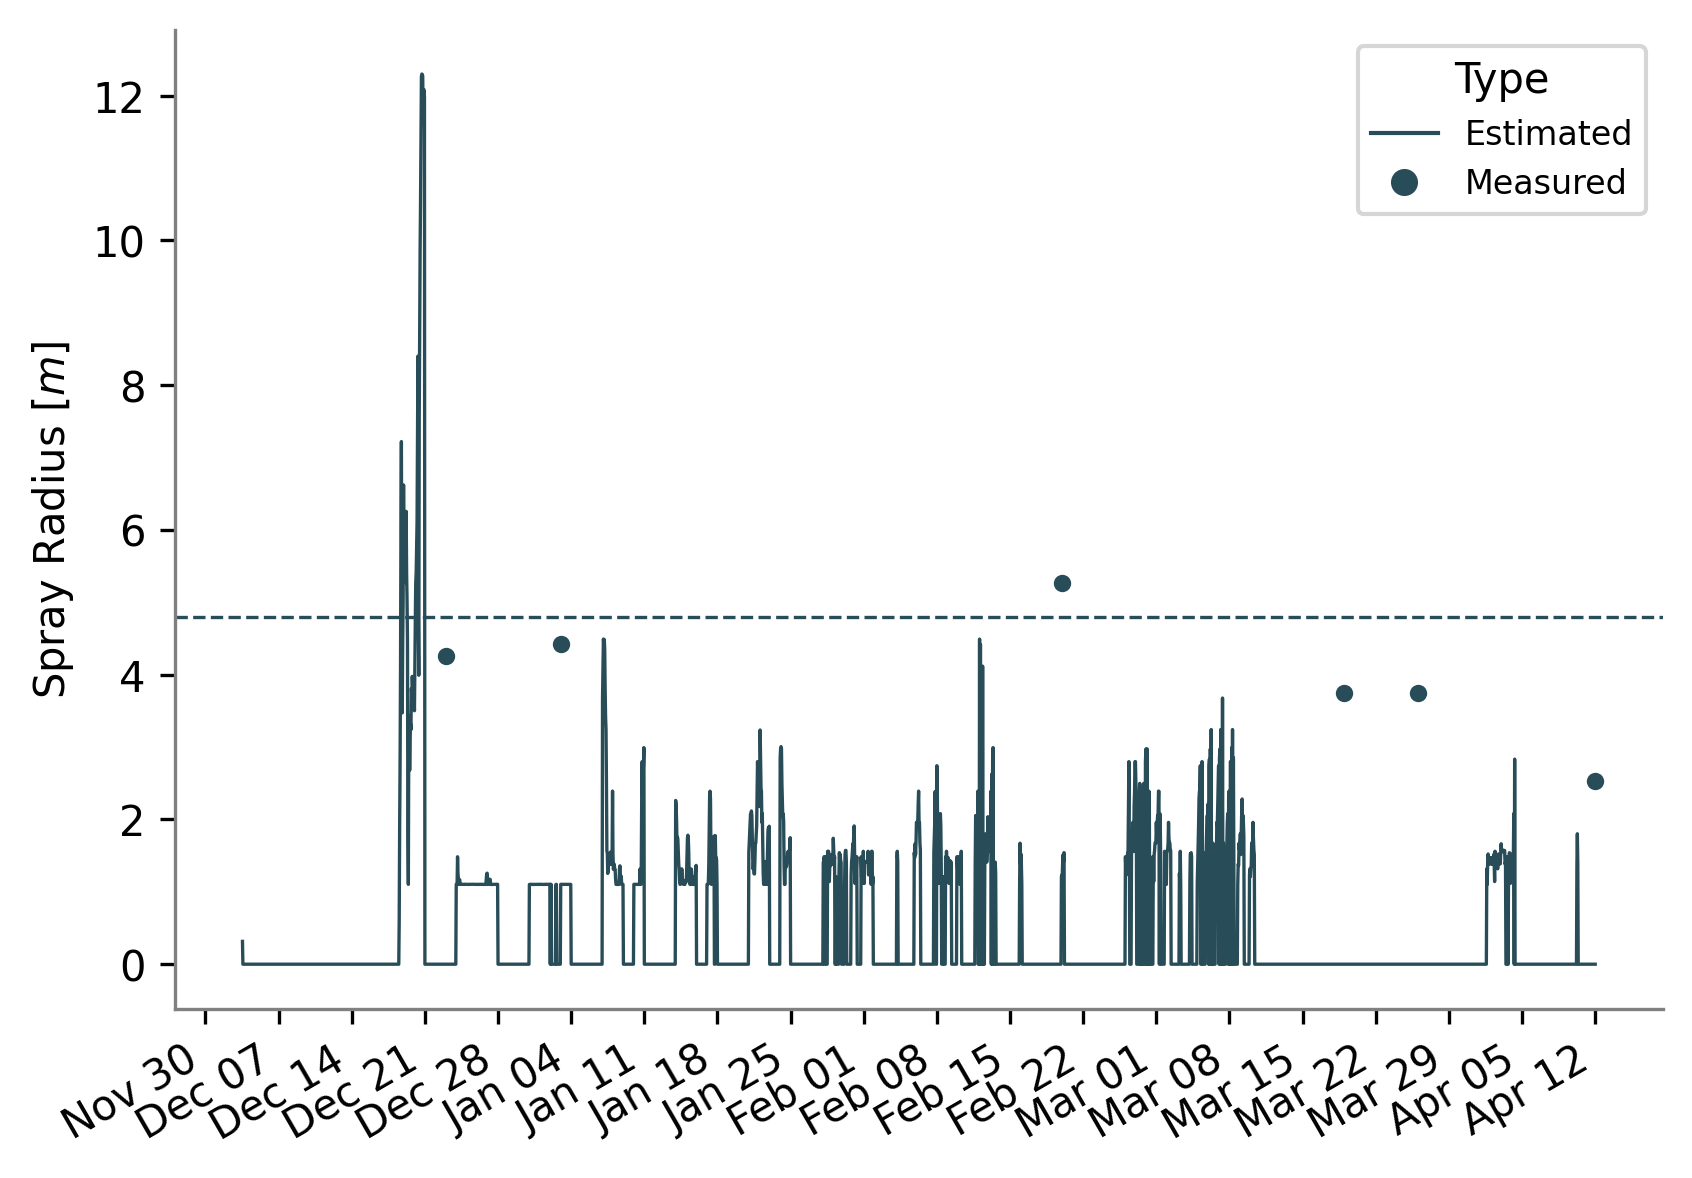
\includegraphics[width=12 cm]{Figures/radf.png}
\caption{Modelled spray radius using wind values from CH22 and CH21 experiments. Measured spray radius values are
indicated as dots.}
\label{fig:wind}
\end{figure*}

\section{Discussion}

\subsection{Implementation of automated construction strategy}

Our strategy is not yet suitable for direct application in current AIR construction sites due to
the cost of the automation system. However, we believe sufficient cost reduction is possible through simpler
automation systems which control only the duration of fountain spray and not their quantity.

Despite the cost, implementation can be reasonable if multiple stupas are constructed simultaneously. In the Guttannen site, for example, eight identical ice stupas could have been constructed
using the water supply of just one traditional ice stupa, thereby increasing eight times the melt water supply.

\subsection{The state of AIR technology}

The present study shows one strategy that can improve the water-use efficiency of AIRs. We chose this strategy because it enables the use the AIR model in a simple and effective manner. Ice stupa construction can significantly be improved with sufficient
engineering expertise. The
fountain nozzle design is crucial for increasing the ice volume obtained. However, no methodology currently
exists to rank the several fountain nozzles used for construction. An ideal pipeline configuration could make
this technology cheaper and maintenance free. However, optimization of the pipeline material and diameters is
yet to be performed---despite the time lost on pipeline freezing events and the potential cost
reduction with cheaper pipeline materials and sizes. Therefore, we strongly encourage the
engineering community to get involved and push the limits of the cost-effectiveness, size, and survival duration of artificial ice
reservoirs. 

\subsection{Additional water losses}

A portion of the water volume exiting the fountains does not reach the ground due to both thermodynamic---evaporation and sublimation---and mechanical---wind-driven redistribution---effects. Although these water losses can
be significant \citep{hanzerSimulationSnowManagement2020}, their simulation with physical formulation is
challenging because this is sensitive to the diameter of the water droplets produced by the fountain.

\conclusions

We compare an automated AIR construction strategy with a traditional one
using data collected in Guttannen, Switzerland and Gangles, India.

The main purpose of the present study is to quantify the influence of different fountain scheduling strategies on the
water-use efficiency and ice volume of AIRs exposed to identical weather conditions. We found that overwatering by
unscheduled fountains not only increased the fountain wastewater production but also enhanced the melting rate
of AIRs, mainly due to surface albedo and fountain heat flux feedbacks. Scheduled fountains, in contrast,
consumed only 13 \% of the unscheduled fountain water supply. However, volume evolution of both AIRs
showed no significant variations. 

Two different model forcing strategies were used to recommend two types of scheduled discharge rates: limited weather windows to favor higher ice volume and water supply
to favor water-use
efficiency. These model versions were able to capture more than 44 \% of the freezing rate
variations of the traditional AIR. Simulations converting several unscheduled fountains to scheduled ones showed
that at least a threefold increase in water-use efficiency is possible without compromising meltwater
production.

The influence of wind-driven redistribution on the spray radius resulted in AIRs 6 times bigger despite 3 $\degree C$ warmer temperatures. This implies that higher wind speed caused the volume
differences in the AIRs constructed at the Swiss location through three consecutive winters.  However, higher wind
speed can also cause water losses if water droplets are distributed beyond the spray radius. Therefore, a
critical wind speed needs to be determined to force wind-driven redistribution to increase spray
radius instead of water losses. Future selection of construction locations and design of automation
algorithms need to capitalize on wind-driven redistribution effects to further increase water-use
efficiency.

Fountain nozzles play an important role in the construction process. First, these consume most of the input water
pressure to form water droplets. Second, their engineering design determines the droplet size distribution and
spray radius. Future research, therefore, must be devoted to engineer fountain nozzles able to create water
droplets with a size distribution that consumes less energy and a trajectory that increases the
spray radius.

\appendix


\section{Model forcing based on water-use efficiency and maximum ice volume objectives} \label{sec:SEB}

We reduced model complexity and data requirement \citep{balasubramanianInfluenceMeteorologicalConditions2022} through assumptions that optimize ice volume (IVOM) or water-use efficiency (WEOM). We define the freezing rate and melting
rate as the positive and negative mass change rate, respectively. We choose assumptions based on whether these
overestimate or underestimate the freezing rate. IVOM assumptions overestimate freezing rate, whereas WEOM
assumptions underestimate freezing rate. We describe these two kinds of assumptions applied on each 
energy balance component: 

\subsection{Surface area $A_{cone}$ assumptions}

Determination of surface area during the accumulation period is achieved by assuming a constant ice cone
radius equal to the fountain spray radius. The surface area scales the freezing rate of the AIR. Hence, for the
IVOM version, we assume the maximum possible slope to be 1 for the ice cone.
Therefore, area is estimated as:  

\begin{equation} A_{cone} =\sqrt{2} \cdot \pi \cdot r_{F}^2  \end{equation}

Similarly, for the water-use efficiency objective, the area of the conical AIR is approximated to the area of
its circular base. Therefore, area is estimated as:

\begin{equation} A_{cone} =\pi \cdot r_{F}^2  \end{equation}

\subsection{Net shortwave radiation \texorpdfstring{$q_{SW}$}{Lg} assumptions}
\label{sec:SW}

The net shortwave radiation $q_{SW}$ is computed as follows:

\begin{equation} 
q_{SW} = (1- \alpha) \cdot ( SW_{direct} \cdot f_{cone} + SW_{diffuse})
\label{eqn:SW} 
\end{equation}

where $\alpha$ is the albedo value, $SW_{direct}$ is the direct shortwave radiation, $SW_{diffuse}$ is the
diffuse shortwave radiation, and $f_{cone}$ is the solar area fraction.

The data requirement was reduced by estimating the global shortwave radiation and pressure using directly the
location's coordinates and altitude through the solar radiation model described in
\citet{holmgrenPvlibPythonPython2018}. The algorithm used to estimate the clear-sky global radiation is
described in \citet{ineichenBroadbandSimplifiedVersion2008}.  

The diffuse and direct shortwave radiation are determined using the estimated global solar radiation as follows:

\begin{equation}
\begin{split}
  SW_{diffuse} &= cld \cdot SW_{global}\\
  SW_{direct} &= (1-cld) \cdot SW_{global}
\end{split}
\end{equation}

where $cld$ is the cloudiness factor. $cld$ is assumed to be 1 and 0 for the water-use efficiency and ice volume
objective, respectively.

We ignore the variations in the albedo and assume it to be equal to snow albedo and ice albedo for the ice
volume and water-use efficiency objective, respectively.

The solar area fraction $f_{cone}$ of the ice structure exposed to the direct shortwave radiation depends on the
shape considered and is computed as:

\begin{equation}
		f_{cone} =\frac{(0.5 \cdot r_{cone} \cdot h_{cone}) \cdot cos \theta_{sun} +(\pi \cdot
			{(r_{cone})}^2/2) \cdot sin \theta_{sun} }{\pi \cdot r_{cone} \cdot ({(r_{cone})}^2+{(h_{cone})}^2)^{1/2}}\\
\end{equation}

For the ice volume objective, we assume the slope of the cone to be 1; $f_{cone}$ is determined as follows:

\begin{equation}
		f_{cone} =\frac{ cos \theta_{sun} + \pi \cdot sin \theta_{sun} }{2\sqrt{2} \cdot \pi }
\end{equation}

Similarly, for the water-use efficiency objective, we assume the slope of the cone to be negligible obtain:

\begin{equation}
		f_{cone} =\frac{ sin \theta_{sun} }{2 }
\end{equation}

\subsection{Net longwave radiation \texorpdfstring{$q_{LW}$}{Lg} assumptions} 

We assume $T_{ice} = 0 \degree C$ to determine outgoing longwave radiation. To
constrain the minimum ice temperature is challenging; therefore, we maintain this assumption for both our objectives. However, to
estimate atmospheric emissivity, we again assume $cld$ to be 1 and 0 for the water-use efficiency and ice volume
objective, respectively.

\subsection{Turbulent fluxes assumptions} \label{sec:Qs}

Turbulent fluxes estimation depends on the slope of the cone through the $\mu_{cone}$ parameter. As suggested 
by \citet{oerlemansBriefCommunicationGrowth2021}, we estimated this parameter as follows:

\begin{equation}
  \mu_{cone} =1 + s_{cone}/2
\end{equation}

Hence, the $\mu_{cone}$ parameter takes values of 1.5 and 1 for the ice volume and water-use efficiency
objective, respectively.  Since turbulent fluxes impact both the freezing and the melting rates, this assumption
may not favor the corresponding objectives for certain sites.

\appendixtables   %% needs to be added in front of appendix tables

\begin{table}
  \caption{Free parameters in the model categorized as constant, model hyperparameters, and weather 
  parameters with their respective values/ranges.}

	\label{tab:parameters}
	\begin{tabular}{lllll}
		\toprule

		\textbf{Constant parameters}                       & \textbf{Symbol} & \textbf{Value} &
    \textbf{Unit} & \textbf{References} \\
    Van Karman constant & $\kappa$      & 0.4        &dimensionless & \citet{cuffeyPhysicsGlaciers2010}              \\
    Stefan Boltzmann constant & $\sigma$ & $\num{5.67 e-8} $& $W\, m^{-2}\, K^{-4}$ & \citet{cuffeyPhysicsGlaciers2010}\\
    Air pressure at sea level & $p_{0,a}$ & 1013 & $hPa$  & \citet{molgAblationAssociatedEnergy2004}\\
    Density of water & $\rho_{w}$ & 1000 & $kg\, m^{-3}$    & \citet{cuffeyPhysicsGlaciers2010}\\
    Density of ice & $\rho_{ice}$ & 917 & $kg\, m^{-3}$ & \citet{cuffeyPhysicsGlaciers2010}\\
    Density of air & $\rho_{a}$ &  1.29 & $kg\, m^{-3}$   & \citet{molgAblationAssociatedEnergy2004}\\
    Specific heat of water & $c_{w}$ & 4186 & $J\, kg^{-1}\,\degree C^{-1}$  & \citet{cuffeyPhysicsGlaciers2010}\\
    Specific heat of ice & $c_{ice}$ & 2097 & $J\, kg^{-1}\,\degree C^{-1}$ & \citet{cuffeyPhysicsGlaciers2010}\\
    Specific heat of air & $c_{a}$ & 1010 & $J\, kg^{-1}\,\degree C^{-1}$ & \citet{molgAblationAssociatedEnergy2004}\\
    Thermal conductivity of ice & $k_{ice}$ & 2.123  & $W\, m^{-1}\, K^{-1}$ & \citet{bonalesThermalConductivityIce2017} \\
    Latent heat of sublimation & $L_{s}$ & \num{2.848e6}  & $J\, kg^{-1}$ &   \citet{cuffeyPhysicsGlaciers2010}\\
    Latent heat of fusion & $L_{f}$ & \num{3.34e5} & $J\, kg^{-1}$ & \citet{cuffeyPhysicsGlaciers2010}\\
    Gravitational acceleration & $g$ & 9.81 & $m\, s^{-2}$ &\citet{cuffeyPhysicsGlaciers2010}\\
    Weather station height & $h_{AWS}$ & 2 & $m$ & assumed \\
    Model timestep                            & $\Delta t$            & $3600$           & $s$ & assumed \\\midrule

		\textbf{Model Hyperparameters} & \textbf{Symbol} & \textbf{Range} & \textbf{Unit} & \textbf{References} \\
    Surface layer thickness             & $\Delta x$            & $[\num{1e-2},\num{1e-1}]$           & $m$ & assumed
    \\\midrule
		\textbf{Weather parameters} & \textbf{Symbol} & \textbf{Range} & \textbf{Unit} & \textbf{References} \\
    Ice emissivity                      & $\epsilon_{ice}$      & $[0.95,0.99]$         & dimensionless & \citet{horiInsituMeasuredSpectral2006}             \\
    Surface roughness                   & $z_0$                 & $[\num{1e-3},\num{5e-3}]$            & $m$  & \citet{brockMeasurementParameterizationAerodynamic2006}       \\
    Ice albedo                          & $\alpha_{ice}$        & $[0.15,0.35]$         & dimensionless  &
    \citet{steinerModellingIcecliffBackwasting2015};            \\
    & &    &  & \citet{zollesRobustUncertaintyAssessment2019}      \\
    Snow albedo                         & $\alpha_{snow}$       & $[0.8,0.9]$        & dimensionless  & \citet{zollesRobustUncertaintyAssessment2019}              \\
    Precipitation temperature threshold & $T_{ppt}$             & $[0,2]$            & $\degree C$& \citet{shichangResponseZhadangGlacier2010}  \\
    Albedo decay rate                   & $\tau$                & $[10,22]$           & $days$ &
    \citet{schmidtImportanceAccurateGlacier2017};      \\
    & &    &  & \citet{oerlemansYearRecordGlobal1998}      \\\midrule
	\end{tabular}
\end{table}
\clearpage


\noappendix 

\authorcontribution{
  \textbf{Suryanarayanan Balasubramanian}: Conceptualization, Methodology, Investigation, Data curation, Visualization, Software,
Writing -- original draft preparation. \textbf{Martin Hoelzle}: Conceptualization, Supervision, Investigation, Writing -- review and editing. \textbf{Roger Waser}: Resources -- automation system, Writing -- review and editing.} %% this section is mandatory

\competinginterests{The authors declare that they have no known competing financial interests or personal
relationships that could have appeared to influence the work reported in this paper.} %% this section is mandatory even if you declare that no competing interests are present

\financialsupport{
This work was supported and funded by the University of Fribourg and by the Swiss Government Excellence Scholarship (SB). The associated fieldwork in Guttannen was funded by the Glaciers Alive Association.
}

\begin{acknowledgements}
This work would not have been possible without the unconditional support of Daniel Bürki from Guttannen Bewegt Association to manage our field experiments for the past three winters. David Sciboz and Maria Gruber helped us install the weather station and the automation system. The smooth operation of the automation system was possible due to the user interface designed by Martin Von Burg. We would particularly like to thank our english editors Ana Rodríguez Crespo and Akshatha N Tirumale. We also thank Dr. Eric Pohl for valuable suggestions that improved the manuscript.
\end{acknowledgements}

\bibliographystyle{copernicus}
\bibliography{zot_refs.bib}

\end{document}
